\documentclass[5p,authoryear,square]{elsarticle}
\makeatletter 
\def\ps@pprintTitle{%
 \let\@oddhead\@empty
 \let\@evenhead\@empty
 \let\@evenfoot\@oddfoot} % Supprimer le bas de page ELSEVIER
\makeatother
\usepackage[utf8]{inputenc} % En unicode
\usepackage[T1]{fontenc}
\usepackage[french]{babel}
\usepackage[babel=true]{csquotes} % permet de faire \enquote{a} (« a »)
\usepackage[fleqn]{amsmath} % pour certains signes mathématiques
\usepackage{amsthm} % Pour \begin{gather}
\usepackage{booktabs} % pour \toprule (un style de tableau)
\usepackage{multirow} % Pour colonnes multiples des tableaux
\usepackage{amssymb} % Pour \leqslant (<=, >=)
\usepackage{float}
\usepackage{subcaption}
\usepackage{xcolor}
\usepackage{cancel}
\usepackage{graphicx}
\usepackage[section]{placeins} % Empêcher les flottants de dépasser la section
\usepackage{dblfloatfix} % Améliorer le placement des figures* en deux colonnes
\graphicspath{{figures/}}
% \definecolor{refcolor}{HTML}{0000FF}        % blue for refs
% \definecolor{citecolor}{HTML}{FF00FF}       % violet/magenta for citations
% \definecolor{footnotecolor}{HTML}{FF00FF}   % magenta for footnotes


%\bibliographystyle{elsarticle-num}
\bibliographystyle{elsarticle-harv}

\usepackage[bookmarks=true,colorlinks=true,linkcolor = red,citecolor=red,urlcolor=red]{hyperref}
\usepackage[french,nameinlink,noabbrev]{cleveref}


\begin{document}

\begin{frontmatter}

\title{\textbf{Modélisation de l'effet dynamique d'un échantillon granulaire lâche par Méthode des Élements Discrètes}}

%% Group authors per affiliation:
\author{Gaël COMBE, Vincent RICHEFEU, Viet Anh QUACH}
\address{Laboratoire 3SR, Université Grenoble Alpes}

% \author{Encadré par Sandra Ulrich Ngueveu}
% \address{LAAS-CNRS, Toulouse}

\begin{abstract}

L'objectif principal de cet article est d'étudier l'influence des effets cinétiques sur un échantillon granulaire lâche soumis à une compression triaxiale, à l'aide de la Méthode des Éléments Discrets (DEM) en régime résiduel.
Pour cela, en plus de la masse définie au niveau des grains, des termes cinétiques supplémentaires sont intégrés dans le calcul DEM.
En particulier, dans le domaine résiduel, la rhéologie $\mu_{\text{résiduel}}(I)$ semble indépendante de ces modifications, pour différentes vitesses de compression (c'est-à-dire différents nombres d'inertie $I$).
Ce travail constitue une pré-étude du comportement d'un volume élémentaire représentatif (VER) en vue de la modélisation d'un écoulement gravitaire couplant la Méthode des Éléments Discrets et la Méthode des Points Matériels.

\end{abstract}

\begin{keyword}
DEM \sep termes dynamiques \sep nombre d'inertie \sep $\mu(I)$ rhéologie \sep échantillon lâche \sep résiduel
\end{keyword}

\end{frontmatter}
% \footnotemark{}.
% \footnotetext{}

%\linenumbers
\section{Introduction}\label{introduction}
La rhéologie $\mu(I)$ caractérise un aspect fondamental dans la modélisation des écoulements granulaires, notamment pour les phénomènes gravitaires.

Actuellement, de nombreuses études bibliographiques détaillées ont été réalisées sur la rhéologie en régime résiduel. Ces travaux constituent une base solide pour la vérification des calculs DEM présentés ici : en extrayant la contrainte dans la zone d’état critique, on la convertit en coefficient de frottement $\mu$ via le critère de Mohr-Coulomb, puis on la compare aux courbes expérimentales issues de la littérature.

Pour mener à bien cette démarche, le modèle DEM utilisé dans ce travail dépasse le cadre quasi-statique dès que $I > 10^{-3}$. Afin d’intégrer les effets dynamiques dans les calculs, des termes cinétiques supplémentaires ont été ajoutés, comme détaillé dans la suite de l’article.
\section{Méthodologie}\label{methode}

\subsection{DEM}\label{dem}

La Méthode des Éléments Discrets (DEM) a été développée pour étudier les problèmes mécaniques des matériaux granulaires et géomatériaux.
Dans cette approche, le milieu granulaire est modélisé comme un assemblage de grains interagissant individuellement.
Dans le contexte de l'homogénéisation multi-échelle, la DEM constitue un bon candidat pour servir de loi constitutive homogénéisée numériquement.

\begin{figure}[h] \centering
	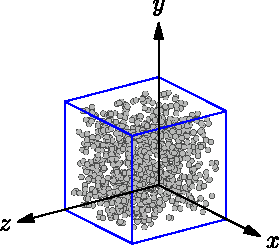
\includegraphics[width=2in]{figures/modele.pdf}
	\caption[]{Modele DEM 3D d'un échantillon lâche (un gaz)}
	\label{echantillon} 
\end{figure}


Dans la modélisation, l’échantillon est soumis à une contrainte de confinement constante selon les directions $x$ et $z$, puis une déformation axiale est appliquée suivant l’axe vertical $y$ (\cref{echantillon}).
L’augmentation progressive de la vitesse de déformation est contrôlée par le nombre d'inertie.


    Le nombre d'inertie $I$ est défini à partir du ``temps d'inertie'' et du ``temps de cisaillement''.
    Le temps d'inertie caractérise la durée de déplacement d'une particule moyenne de masse $m$ et de diamètre $d$, sous la pression $P$, en $D$ dimensions\footnote{\citep{combe2023demlecture}}. Leurs expressions sont :
    \begin{align}
        	\tau_c &= \dfrac{1}{\dot{\epsilon}} = \dfrac{v}{H_0}, \\
        	\tau_i &= \sqrt{\dfrac{m}{P.d^{D-2}}}
    \end{align}

    Dans notre cas (compression triaxiale en 3D, $D=3$) on obtient :
    \begin{align}
        I &= \dfrac{\tau_i}{\tau_c}
        = \dot{\epsilon}\ \sqrt{\dfrac{m}{\sigma_0.d}}
        = \dfrac{v}{H_0}\,\sqrt{\dfrac{\tfrac{4}{3}\pi R^3 \rho}{\sigma_{0}.2R}}
    \end{align}

    Où :
    \begin{itemize}
        \item $v$ : vitesse de compression,
        \item $H_0$ : hauteur initiale de l'échantillon,
        \item $R$ : rayon moyen des particules,
        \item $\rho$ : masse volumique des particules,
        \item $\sigma_{0}$ : contrainte de confinement
    \end{itemize}

\begin{table}[htbp]
\centering
\footnotesize
\begin{tabular}{@{}llll@{}}
\toprule
\textbf{Symbole} & \textbf{Paramètre} & \textbf{Valeur} & \textbf{Unité} \\
\midrule
N & Nombre de particules & $1000 \div 3375$ &  \\
R & Rayon des particules & $3 \div 5 $& mm \\
$\rho$ & Masse volumique & 2500 & kg/m$^3$ \\
$\sigma_{xx} = \sigma_{zz}$ & Contrainte isotrope & 30 & kPa \\
$k_n$, $k_t$ & Raideur norm./tang. & $3 \times 10^6$ & N/m \\
$\kappa$ & Niveau de raideur & 6250 &  \\
$\mu$ & Coefficient de frottement & 0.5 &  \\
$d_t$ & Pas de temps & $10^{-6} \div 10^{-9}$ & s \\
$\alpha$ & Coefficient d'amortissement & 0 &  \\
I & Nombre d'inertie & $10^{-4} \div 10^{-1}$ &  \\
\bottomrule
\end{tabular}
\caption{Paramètres utilisés dans la modélisation compression triaxiale DEM}
\label{parametres_triaxiale}
\end{table}



\subsection{Rhéologie}\label{rheologie}

À l'échelle macroscopique, la rhéologie $\mu(I)$ joue un rôle crucial dans la description des écoulements granulaires. Elle établit une relation constitutive entre le tenseur des contraintes du flux et le tenseur des taux de déformation  \cite{jop2006constitutive} :
\begin{equation}
\sigma_{ij} = -P \delta_{ij} + \mu(I) P \frac{\dot{\gamma}_{ij}}{\lVert \dot{\gamma} \rVert}
\label{flowTensor}
\end{equation}
où :
\begin{equation}
\mu(I) = \mu_s + \dfrac{\mu_2 - \mu_s}{1 + \dfrac{I_0}{I}}
\label{muI}
\end{equation}

La fraction solide caractérise la dispersion des particules solides $V_s$ dans un volume $V$ : $\Phi = V_s/V$..  
Leur evolution est prescrit égalementen fonction du $I$ comme suivant  
\begin{equation}
\Phi(I) = \Phi^{\max} - bI
\label{phiI}
\end{equation}

où: $\mu_s,\ \mu_2,\ I_0,\ \Phi_{\text{max}},\ b $ sont les coefficients empiriques

\subsection{Termes Cinétiques}\label{termeCinetique}
Seuls deux problèmes, à notre connaissance, appartiennent à cette catégorie, 
thus dans le programme PBC3D, 2 termes cinétiques a été ajouté  dans la formulation de calcul:


Dans le calcul de la vrai accélération: 
\begin{equation}
\ddot{s} = h^{-1}(\ddot{r} - \textcolor{red}{2\dot{h}\dot{s}} - \cancel{\ddot{h}s})
    \label{vraiAcc}
\end{equation}	


Et dans le calcul stress tensor: 
\begin{equation}
    \sigma_p = -\frac{1}{|\det h_p|} \left( \sum_k f_k \otimes \ell_k + \textcolor{red}{\sum_n m_n \dot{r}_n \otimes \dot{r}_n} \right) \\
    \label{contrainteDynamique}
\end{equation}	
    où: $\dot{r_n} = \textcolor{red}{h\dot{s}} + \cancel{\dot{h}s}$

the first term denotes Love-Weber stress, while the
second (kinetic) term may become significant during extremely rapid deformations

Les champs cancle dans l'équation sont des champs affine, jetant pour garder seulement des composants de fluctuation.
Un petit différence ($\sqrt{\frac{\pi}{6}}$) dans la notion de nombre d'ienrtie DEM et mobobilisation d'écoulement:
\begin{equation}
    I = \dot{\varepsilon} \times \sqrt{\frac{m}{\sigma_{33} \times \bar{a}}}
 = \sqrt{\frac{\pi}{6}} \times \frac{\dot{\varepsilon} .\bar{a}}{\sqrt{\sigma_{33}/\rho_s}}
    \label{comparerO}
\end{equation}



\subsection{Critère de rupture de Mohr} \label{Mohr}
Dans le sable sec, autre dire sans cohésif, les interactions entre les particules sont purement frottant. 
On utilise le critère de Mohr pour évaluer le compotment à l'échelle microscopic à l'echelle macroscopic.
Dans le cas simplicité, l'enveloppe de Mohr est simplifié par un droit transversale tous les cercles de Mohr.
La résistance au force de cissailement du matériau est composant de deux indices: le valeur $\mu = \tan(\phi)$, calculé selon l'angle de frottement $\phi$ de la droit et la cohésion apparente $C$, qui est est la intersection entre la droit avec l'axe y (i.e l'axe de cissailement)
Un point particulier de la méthode DEM est que l'on agit uniquement sur les paramètres microscopiques, alors que les comportements à grande échelle émergent naturellement.  
Cette propriété peut être vérifiée en comparant avec les comportements macroscopiques bien connus en mécanique des sols.  

Le cercle de Mohr est une méthode bien connue pour identifier la résistance au cisaillement maximale du sol.  
À partir de ses courbes, on peut déterminer la cohésion $c$ et l'angle de frottement interne $\varphi$ selon la relation:
\begin{equation}
    \tau = \sigma_n \tan(\varphi) + c
    \label{eq:tangentMohr}
\end{equation}
La pente de la droite tangente aux cercles, soit $\tan(\varphi) = \mu$, reflète le frottement interne à l'état considéré.  
Le $\mu_{\text{résiduel}}$ correspond à la pente de la droite tangente au cercle de Mohr à l'état critique.  
On considère généralement que ce $\mu_{\text{résiduel}}$ est une valeur stationnaire.  
Dans notre cas, le matériau étudié est du sable sec. Le point d'intersection entre la droite tangente aux cercles et l'axe vertical, selon la théorie, doit être nul, ce qui correspond à une cohésion nulle ($c=0$).

\section{Résultat et discussion}\label{resultat}

\subsection{Nombre des particules}\label{N}

\begin{figure}[htbp]
    \centering
    \scalebox{0.5}{% GNUPLOT: LaTeX picture with Postscript
\begingroup
  \makeatletter
  \providecommand\color[2][]{%
    \GenericError{(gnuplot) \space\space\space\@spaces}{%
      Package color not loaded in conjunction with
      terminal option `colourtext'%
    }{See the gnuplot documentation for explanation.%
    }{Either use 'blacktext' in gnuplot or load the package
      color.sty in LaTeX.}%
    \renewcommand\color[2][]{}%
  }%
  \providecommand\includegraphics[2][]{%
    \GenericError{(gnuplot) \space\space\space\@spaces}{%
      Package graphicx or graphics not loaded%
    }{See the gnuplot documentation for explanation.%
    }{The gnuplot epslatex terminal needs graphicx.sty or graphics.sty.}%
    \renewcommand\includegraphics[2][]{}%
  }%
  \providecommand\rotatebox[2]{#2}%
  \@ifundefined{ifGPcolor}{%
    \newif\ifGPcolor
    \GPcolortrue
  }{}%
  \@ifundefined{ifGPblacktext}{%
    \newif\ifGPblacktext
    \GPblacktextfalse
  }{}%
  % define a \g@addto@macro without @ in the name:
  \let\gplgaddtomacro\g@addto@macro
  % define empty templates for all commands taking text:
  \gdef\gplbacktext{}%
  \gdef\gplfronttext{}%
  \makeatother
  \ifGPblacktext
    % no textcolor at all
    \def\colorrgb#1{}%
    \def\colorgray#1{}%
  \else
    % gray or color?
    \ifGPcolor
      \def\colorrgb#1{\color[rgb]{#1}}%
      \def\colorgray#1{\color[gray]{#1}}%
      \expandafter\def\csname LTw\endcsname{\color{white}}%
      \expandafter\def\csname LTb\endcsname{\color{black}}%
      \expandafter\def\csname LTa\endcsname{\color{black}}%
      \expandafter\def\csname LT0\endcsname{\color[rgb]{1,0,0}}%
      \expandafter\def\csname LT1\endcsname{\color[rgb]{0,1,0}}%
      \expandafter\def\csname LT2\endcsname{\color[rgb]{0,0,1}}%
      \expandafter\def\csname LT3\endcsname{\color[rgb]{1,0,1}}%
      \expandafter\def\csname LT4\endcsname{\color[rgb]{0,1,1}}%
      \expandafter\def\csname LT5\endcsname{\color[rgb]{1,1,0}}%
      \expandafter\def\csname LT6\endcsname{\color[rgb]{0,0,0}}%
      \expandafter\def\csname LT7\endcsname{\color[rgb]{1,0.3,0}}%
      \expandafter\def\csname LT8\endcsname{\color[rgb]{0.5,0.5,0.5}}%
    \else
      % gray
      \def\colorrgb#1{\color{black}}%
      \def\colorgray#1{\color[gray]{#1}}%
      \expandafter\def\csname LTw\endcsname{\color{white}}%
      \expandafter\def\csname LTb\endcsname{\color{black}}%
      \expandafter\def\csname LTa\endcsname{\color{black}}%
      \expandafter\def\csname LT0\endcsname{\color{black}}%
      \expandafter\def\csname LT1\endcsname{\color{black}}%
      \expandafter\def\csname LT2\endcsname{\color{black}}%
      \expandafter\def\csname LT3\endcsname{\color{black}}%
      \expandafter\def\csname LT4\endcsname{\color{black}}%
      \expandafter\def\csname LT5\endcsname{\color{black}}%
      \expandafter\def\csname LT6\endcsname{\color{black}}%
      \expandafter\def\csname LT7\endcsname{\color{black}}%
      \expandafter\def\csname LT8\endcsname{\color{black}}%
    \fi
  \fi
    \setlength{\unitlength}{0.0500bp}%
    \ifx\gptboxheight\undefined%
      \newlength{\gptboxheight}%
      \newlength{\gptboxwidth}%
      \newsavebox{\gptboxtext}%
    \fi%
    \setlength{\fboxrule}{0.5pt}%
    \setlength{\fboxsep}{1pt}%
    \definecolor{tbcol}{rgb}{1,1,1}%
\begin{picture}(7200.00,5040.00)%
    \gplgaddtomacro\gplbacktext{%
      \csname LTb\endcsname%%
      \put(814,1364){\makebox(0,0)[r]{\strut{}$0$}}%
      \csname LTb\endcsname%%
      \put(814,2055){\makebox(0,0)[r]{\strut{}$50$}}%
      \csname LTb\endcsname%%
      \put(814,2746){\makebox(0,0)[r]{\strut{}$100$}}%
      \csname LTb\endcsname%%
      \put(814,3437){\makebox(0,0)[r]{\strut{}$150$}}%
      \csname LTb\endcsname%%
      \put(814,4128){\makebox(0,0)[r]{\strut{}$200$}}%
      \csname LTb\endcsname%%
      \put(814,4819){\makebox(0,0)[r]{\strut{}$250$}}%
      \csname LTb\endcsname%%
      \put(946,1144){\makebox(0,0){\strut{}$0$}}%
      \csname LTb\endcsname%%
      \put(1922,1144){\makebox(0,0){\strut{}$10$}}%
      \csname LTb\endcsname%%
      \put(2898,1144){\makebox(0,0){\strut{}$20$}}%
      \csname LTb\endcsname%%
      \put(3875,1144){\makebox(0,0){\strut{}$30$}}%
      \csname LTb\endcsname%%
      \put(4851,1144){\makebox(0,0){\strut{}$40$}}%
      \csname LTb\endcsname%%
      \put(5827,1144){\makebox(0,0){\strut{}$50$}}%
      \csname LTb\endcsname%%
      \put(6803,1144){\makebox(0,0){\strut{}$60$}}%
    }%
    \gplgaddtomacro\gplfronttext{%
      \csname LTb\endcsname%%
      \put(341,3091){\rotatebox{-270}{\makebox(0,0){\strut{}$\widehat{\text{q}}$ (kPa)}}}%
      \put(3874,814){\makebox(0,0){\strut{}$\varepsilon_{yy}$ (\%)}}%
      \csname LTb\endcsname%%
      \put(3019,613){\makebox(0,0)[r]{\strut{}$N = 1000, I = 10^{-1}$}}%
      \csname LTb\endcsname%%
      \put(3019,393){\makebox(0,0)[r]{\strut{}$N = 1000, I = 10^{-3}$}}%
      \csname LTb\endcsname%%
      \put(3019,173){\makebox(0,0)[r]{\strut{}$N = 1000, I = 10^{-2}$}}%
      \csname LTb\endcsname%%
      \put(6250,613){\makebox(0,0)[r]{\strut{}$N = 3375, I = 10^{-1}$}}%
      \csname LTb\endcsname%%
      \put(6250,393){\makebox(0,0)[r]{\strut{}$N = 3375, I = 10^{-2}$}}%
      \csname LTb\endcsname%%
      \put(6250,173){\makebox(0,0)[r]{\strut{}$N = 3375, I = 10^{-3}$}}%
    }%
    \gplbacktext
    \put(0,0){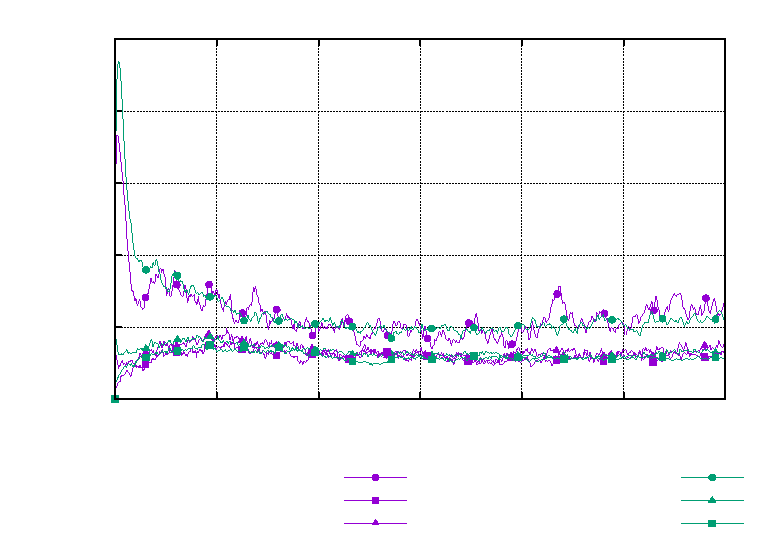
\includegraphics[width={360.00bp},height={252.00bp}]{./ComparerNP}}%
    \gplfronttext
  \end{picture}%
\endgroup
}
    \caption{Influence du nombre de particules sur la contrainte résiduelle}
    \label{comparerNP}
\end{figure}

Comme on l'observe sur la \cref{comparerNP}, à l'exception du pic, la contrainte dans le régime résiduel n'est pas affectée par le nombre de particules, et donc par $\mu_{\text{résiduel}}$.
En revanche, un saut de contrainte au pic (régime transitoire) est observé et mérite d'être approfondi, indiquant que $\mu_{\text{transitoire}}$ varie selon le nombre de particules.

\subsection{Influence de termes dynamiques ajouté}\label{termeDynamique}

\Cref{3000_kinetic_q,3000_kinetic_ev} montrent que l'influence des termes cinétiques est négligeable lorsque seuls les champs de fluctuations sont pris en compte.
\begin{figure}[htbp]
    \centering
    \begin{subfigure}{0.45\textwidth}
        \centering
        \scalebox{0.5}{% GNUPLOT: LaTeX picture with Postscript
\begingroup
  \makeatletter
  \providecommand\color[2][]{%
    \GenericError{(gnuplot) \space\space\space\@spaces}{%
      Package color not loaded in conjunction with
      terminal option `colourtext'%
    }{See the gnuplot documentation for explanation.%
    }{Either use 'blacktext' in gnuplot or load the package
      color.sty in LaTeX.}%
    \renewcommand\color[2][]{}%
  }%
  \providecommand\includegraphics[2][]{%
    \GenericError{(gnuplot) \space\space\space\@spaces}{%
      Package graphicx or graphics not loaded%
    }{See the gnuplot documentation for explanation.%
    }{The gnuplot epslatex terminal needs graphicx.sty or graphics.sty.}%
    \renewcommand\includegraphics[2][]{}%
  }%
  \providecommand\rotatebox[2]{#2}%
  \@ifundefined{ifGPcolor}{%
    \newif\ifGPcolor
    \GPcolortrue
  }{}%
  \@ifundefined{ifGPblacktext}{%
    \newif\ifGPblacktext
    \GPblacktextfalse
  }{}%
  % define a \g@addto@macro without @ in the name:
  \let\gplgaddtomacro\g@addto@macro
  % define empty templates for all commands taking text:
  \gdef\gplbacktext{}%
  \gdef\gplfronttext{}%
  \makeatother
  \ifGPblacktext
    % no textcolor at all
    \def\colorrgb#1{}%
    \def\colorgray#1{}%
  \else
    % gray or color?
    \ifGPcolor
      \def\colorrgb#1{\color[rgb]{#1}}%
      \def\colorgray#1{\color[gray]{#1}}%
      \expandafter\def\csname LTw\endcsname{\color{white}}%
      \expandafter\def\csname LTb\endcsname{\color{black}}%
      \expandafter\def\csname LTa\endcsname{\color{black}}%
      \expandafter\def\csname LT0\endcsname{\color[rgb]{1,0,0}}%
      \expandafter\def\csname LT1\endcsname{\color[rgb]{0,1,0}}%
      \expandafter\def\csname LT2\endcsname{\color[rgb]{0,0,1}}%
      \expandafter\def\csname LT3\endcsname{\color[rgb]{1,0,1}}%
      \expandafter\def\csname LT4\endcsname{\color[rgb]{0,1,1}}%
      \expandafter\def\csname LT5\endcsname{\color[rgb]{1,1,0}}%
      \expandafter\def\csname LT6\endcsname{\color[rgb]{0,0,0}}%
      \expandafter\def\csname LT7\endcsname{\color[rgb]{1,0.3,0}}%
      \expandafter\def\csname LT8\endcsname{\color[rgb]{0.5,0.5,0.5}}%
    \else
      % gray
      \def\colorrgb#1{\color{black}}%
      \def\colorgray#1{\color[gray]{#1}}%
      \expandafter\def\csname LTw\endcsname{\color{white}}%
      \expandafter\def\csname LTb\endcsname{\color{black}}%
      \expandafter\def\csname LTa\endcsname{\color{black}}%
      \expandafter\def\csname LT0\endcsname{\color{black}}%
      \expandafter\def\csname LT1\endcsname{\color{black}}%
      \expandafter\def\csname LT2\endcsname{\color{black}}%
      \expandafter\def\csname LT3\endcsname{\color{black}}%
      \expandafter\def\csname LT4\endcsname{\color{black}}%
      \expandafter\def\csname LT5\endcsname{\color{black}}%
      \expandafter\def\csname LT6\endcsname{\color{black}}%
      \expandafter\def\csname LT7\endcsname{\color{black}}%
      \expandafter\def\csname LT8\endcsname{\color{black}}%
    \fi
  \fi
    \setlength{\unitlength}{0.0500bp}%
    \ifx\gptboxheight\undefined%
      \newlength{\gptboxheight}%
      \newlength{\gptboxwidth}%
      \newsavebox{\gptboxtext}%
    \fi%
    \setlength{\fboxrule}{0.5pt}%
    \setlength{\fboxsep}{1pt}%
    \definecolor{tbcol}{rgb}{1,1,1}%
\begin{picture}(7200.00,5040.00)%
    \gplgaddtomacro\gplbacktext{%
      \csname LTb\endcsname%%
      \put(814,704){\makebox(0,0)[r]{\strut{}$0$}}%
      \put(814,1218){\makebox(0,0)[r]{\strut{}$20$}}%
      \put(814,1733){\makebox(0,0)[r]{\strut{}$40$}}%
      \put(814,2247){\makebox(0,0)[r]{\strut{}$60$}}%
      \put(814,2762){\makebox(0,0)[r]{\strut{}$80$}}%
      \put(814,3276){\makebox(0,0)[r]{\strut{}$100$}}%
      \put(814,3790){\makebox(0,0)[r]{\strut{}$120$}}%
      \put(814,4305){\makebox(0,0)[r]{\strut{}$140$}}%
      \put(814,4819){\makebox(0,0)[r]{\strut{}$160$}}%
      \put(946,484){\makebox(0,0){\strut{}$0$}}%
      \put(1922,484){\makebox(0,0){\strut{}$10$}}%
      \put(2898,484){\makebox(0,0){\strut{}$20$}}%
      \put(3875,484){\makebox(0,0){\strut{}$30$}}%
      \put(4851,484){\makebox(0,0){\strut{}$40$}}%
      \put(5827,484){\makebox(0,0){\strut{}$50$}}%
      \put(6803,484){\makebox(0,0){\strut{}$60$}}%
    }%
    \gplgaddtomacro\gplfronttext{%
      \csname LTb\endcsname%%
      \put(341,2761){\rotatebox{-270}{\makebox(0,0){\strut{}q (kPa)}}}%
      \put(3874,154){\makebox(0,0){\strut{}$\varepsilon_{yy}$ (\%)}}%
      \csname LTb\endcsname%%
      \put(5888,4636){\makebox(0,0)[r]{\strut{}$I = 10^{-3}$ cinétique}}%
      \csname LTb\endcsname%%
      \put(5888,4396){\makebox(0,0)[r]{\strut{}$I = 10^{-3}$ sans cinétique}}%
      \csname LTb\endcsname%%
      \put(5888,4156){\makebox(0,0)[r]{\strut{}$I = 10^{-2}$ cinétique}}%
      \csname LTb\endcsname%%
      \put(5888,3916){\makebox(0,0)[r]{\strut{}$I = 10^{-2}$ sans cinétique}}%
      \csname LTb\endcsname%%
      \put(5888,3676){\makebox(0,0)[r]{\strut{}$I = 10^{-1}$ cinétique}}%
      \csname LTb\endcsname%%
      \put(5888,3436){\makebox(0,0)[r]{\strut{}$I = 10^{-1}$ sans cinétique}}%
    }%
    \gplbacktext
    \put(0,0){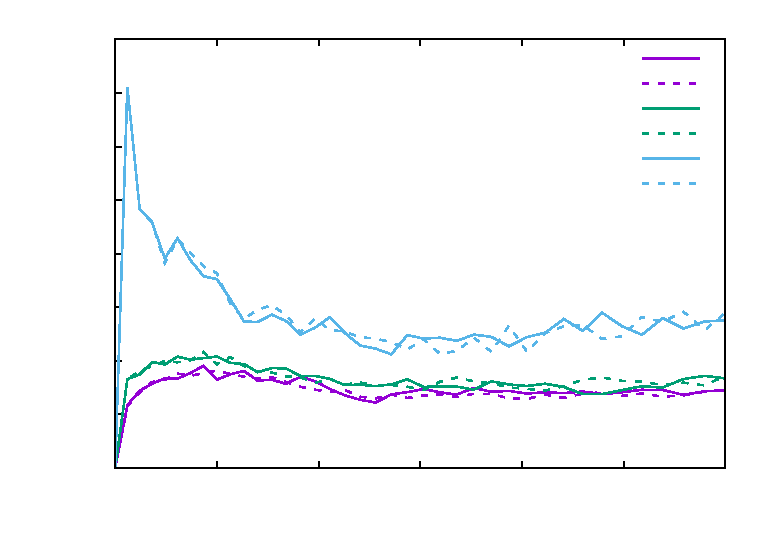
\includegraphics[width={360.00bp},height={252.00bp}]{./3000KineticComp_q}}%
    \gplfronttext
  \end{picture}%
\endgroup
}
        \caption{Contrainte déviatorique}
        \label{3000_kinetic_q}
    \end{subfigure}
    \hfill
    \begin{subfigure}{0.45\textwidth}
        \centering
        \scalebox{0.5}{% GNUPLOT: LaTeX picture with Postscript
\begingroup
  \makeatletter
  \providecommand\color[2][]{%
    \GenericError{(gnuplot) \space\space\space\@spaces}{%
      Package color not loaded in conjunction with
      terminal option `colourtext'%
    }{See the gnuplot documentation for explanation.%
    }{Either use 'blacktext' in gnuplot or load the package
      color.sty in LaTeX.}%
    \renewcommand\color[2][]{}%
  }%
  \providecommand\includegraphics[2][]{%
    \GenericError{(gnuplot) \space\space\space\@spaces}{%
      Package graphicx or graphics not loaded%
    }{See the gnuplot documentation for explanation.%
    }{The gnuplot epslatex terminal needs graphicx.sty or graphics.sty.}%
    \renewcommand\includegraphics[2][]{}%
  }%
  \providecommand\rotatebox[2]{#2}%
  \@ifundefined{ifGPcolor}{%
    \newif\ifGPcolor
    \GPcolortrue
  }{}%
  \@ifundefined{ifGPblacktext}{%
    \newif\ifGPblacktext
    \GPblacktextfalse
  }{}%
  % define a \g@addto@macro without @ in the name:
  \let\gplgaddtomacro\g@addto@macro
  % define empty templates for all commands taking text:
  \gdef\gplbacktext{}%
  \gdef\gplfronttext{}%
  \makeatother
  \ifGPblacktext
    % no textcolor at all
    \def\colorrgb#1{}%
    \def\colorgray#1{}%
  \else
    % gray or color?
    \ifGPcolor
      \def\colorrgb#1{\color[rgb]{#1}}%
      \def\colorgray#1{\color[gray]{#1}}%
      \expandafter\def\csname LTw\endcsname{\color{white}}%
      \expandafter\def\csname LTb\endcsname{\color{black}}%
      \expandafter\def\csname LTa\endcsname{\color{black}}%
      \expandafter\def\csname LT0\endcsname{\color[rgb]{1,0,0}}%
      \expandafter\def\csname LT1\endcsname{\color[rgb]{0,1,0}}%
      \expandafter\def\csname LT2\endcsname{\color[rgb]{0,0,1}}%
      \expandafter\def\csname LT3\endcsname{\color[rgb]{1,0,1}}%
      \expandafter\def\csname LT4\endcsname{\color[rgb]{0,1,1}}%
      \expandafter\def\csname LT5\endcsname{\color[rgb]{1,1,0}}%
      \expandafter\def\csname LT6\endcsname{\color[rgb]{0,0,0}}%
      \expandafter\def\csname LT7\endcsname{\color[rgb]{1,0.3,0}}%
      \expandafter\def\csname LT8\endcsname{\color[rgb]{0.5,0.5,0.5}}%
    \else
      % gray
      \def\colorrgb#1{\color{black}}%
      \def\colorgray#1{\color[gray]{#1}}%
      \expandafter\def\csname LTw\endcsname{\color{white}}%
      \expandafter\def\csname LTb\endcsname{\color{black}}%
      \expandafter\def\csname LTa\endcsname{\color{black}}%
      \expandafter\def\csname LT0\endcsname{\color{black}}%
      \expandafter\def\csname LT1\endcsname{\color{black}}%
      \expandafter\def\csname LT2\endcsname{\color{black}}%
      \expandafter\def\csname LT3\endcsname{\color{black}}%
      \expandafter\def\csname LT4\endcsname{\color{black}}%
      \expandafter\def\csname LT5\endcsname{\color{black}}%
      \expandafter\def\csname LT6\endcsname{\color{black}}%
      \expandafter\def\csname LT7\endcsname{\color{black}}%
      \expandafter\def\csname LT8\endcsname{\color{black}}%
    \fi
  \fi
    \setlength{\unitlength}{0.0500bp}%
    \ifx\gptboxheight\undefined%
      \newlength{\gptboxheight}%
      \newlength{\gptboxwidth}%
      \newsavebox{\gptboxtext}%
    \fi%
    \setlength{\fboxrule}{0.5pt}%
    \setlength{\fboxsep}{1pt}%
    \definecolor{tbcol}{rgb}{1,1,1}%
\begin{picture}(7200.00,5040.00)%
    \gplgaddtomacro\gplbacktext{%
      \csname LTb\endcsname%%
      \put(682,704){\makebox(0,0)[r]{\strut{}$-2$}}%
      \put(682,1078){\makebox(0,0)[r]{\strut{}$-1$}}%
      \put(682,1452){\makebox(0,0)[r]{\strut{}$0$}}%
      \put(682,1826){\makebox(0,0)[r]{\strut{}$1$}}%
      \put(682,2200){\makebox(0,0)[r]{\strut{}$2$}}%
      \put(682,2574){\makebox(0,0)[r]{\strut{}$3$}}%
      \put(682,2949){\makebox(0,0)[r]{\strut{}$4$}}%
      \put(682,3323){\makebox(0,0)[r]{\strut{}$5$}}%
      \put(682,3697){\makebox(0,0)[r]{\strut{}$6$}}%
      \put(682,4071){\makebox(0,0)[r]{\strut{}$7$}}%
      \put(682,4445){\makebox(0,0)[r]{\strut{}$8$}}%
      \put(682,4819){\makebox(0,0)[r]{\strut{}$9$}}%
      \put(814,484){\makebox(0,0){\strut{}$0$}}%
      \put(1812,484){\makebox(0,0){\strut{}$10$}}%
      \put(2810,484){\makebox(0,0){\strut{}$20$}}%
      \put(3809,484){\makebox(0,0){\strut{}$30$}}%
      \put(4807,484){\makebox(0,0){\strut{}$40$}}%
      \put(5805,484){\makebox(0,0){\strut{}$50$}}%
      \put(6803,484){\makebox(0,0){\strut{}$60$}}%
    }%
    \gplgaddtomacro\gplfronttext{%
      \csname LTb\endcsname%%
      \put(341,2761){\rotatebox{-270}{\makebox(0,0){\strut{}$\varepsilon_v$ (\%)}}}%
      \put(3808,154){\makebox(0,0){\strut{}$\varepsilon_{yy}$ (\%)}}%
    }%
    \gplbacktext
    \put(0,0){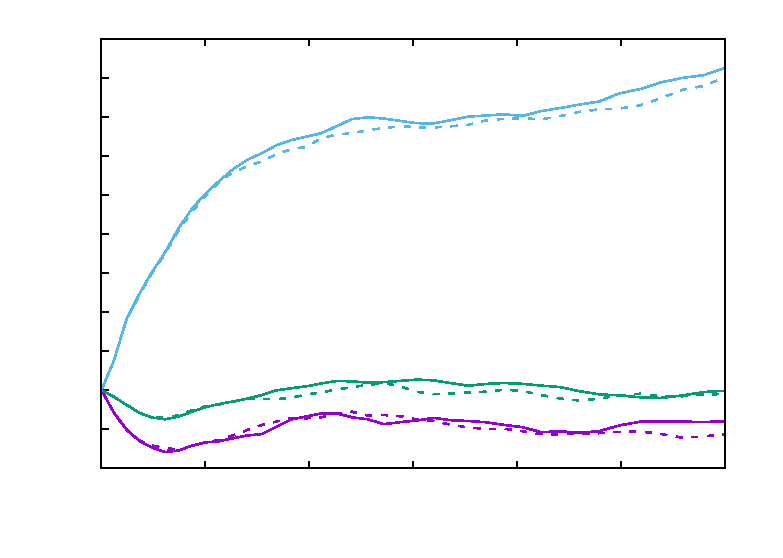
\includegraphics[width={360.00bp},height={252.00bp}]{./3000KineticComp_ev}}%
    \gplfronttext
  \end{picture}%
\endgroup
}
        \caption{Déformation volumique}
        \label{3000_kinetic_ev}
    \end{subfigure}
    \caption{Effet des termes cinétiques sur la réponse mécanique pour $N=3000$. L'influence est négligeable dans le régime de fluctuations.}
    \label{3000_kinetic_comp}
\end{figure}

\subsection{Comportement microscopique à macroscopique}\label{figureMuy}

Étant donné que le sable est purement frottant, l'étude macroscopique via le critère de Mohr est suffisante pour caractériser le comportement à l'état critique.
Un essai d'extension supplémentaire est également modélisé pour vérifier la condition de cohésion nulle, car l'angle de frottement à l'état critique est identique en compression et en extension \citep{gens1982degree}.
En combinant les valeurs de $\sigma_1^{\text{résiduel}}$ et $\sigma_3^{\text{résiduel}}$ issues des deux procédures précédentes, la pente des cercles de Mohr est tracée (\cref{3000_Mohr}), montrant que la cohésion est quasiment nulle et confirmant que l'angle de frottement $\Phi$ varie avec le nombre d'inertie $I$.

\begin{figure}[htbp]
    \centering
    \begin{subfigure}[b]{0.45\textwidth}
        \centering
        \scalebox{0.5}{% GNUPLOT: LaTeX picture with Postscript
\begingroup
  \makeatletter
  \providecommand\color[2][]{%
    \GenericError{(gnuplot) \space\space\space\@spaces}{%
      Package color not loaded in conjunction with
      terminal option `colourtext'%
    }{See the gnuplot documentation for explanation.%
    }{Either use 'blacktext' in gnuplot or load the package
      color.sty in LaTeX.}%
    \renewcommand\color[2][]{}%
  }%
  \providecommand\includegraphics[2][]{%
    \GenericError{(gnuplot) \space\space\space\@spaces}{%
      Package graphicx or graphics not loaded%
    }{See the gnuplot documentation for explanation.%
    }{The gnuplot epslatex terminal needs graphicx.sty or graphics.sty.}%
    \renewcommand\includegraphics[2][]{}%
  }%
  \providecommand\rotatebox[2]{#2}%
  \@ifundefined{ifGPcolor}{%
    \newif\ifGPcolor
    \GPcolortrue
  }{}%
  \@ifundefined{ifGPblacktext}{%
    \newif\ifGPblacktext
    \GPblacktextfalse
  }{}%
  % define a \g@addto@macro without @ in the name:
  \let\gplgaddtomacro\g@addto@macro
  % define empty templates for all commands taking text:
  \gdef\gplbacktext{}%
  \gdef\gplfronttext{}%
  \makeatother
  \ifGPblacktext
    % no textcolor at all
    \def\colorrgb#1{}%
    \def\colorgray#1{}%
  \else
    % gray or color?
    \ifGPcolor
      \def\colorrgb#1{\color[rgb]{#1}}%
      \def\colorgray#1{\color[gray]{#1}}%
      \expandafter\def\csname LTw\endcsname{\color{white}}%
      \expandafter\def\csname LTb\endcsname{\color{black}}%
      \expandafter\def\csname LTa\endcsname{\color{black}}%
      \expandafter\def\csname LT0\endcsname{\color[rgb]{1,0,0}}%
      \expandafter\def\csname LT1\endcsname{\color[rgb]{0,1,0}}%
      \expandafter\def\csname LT2\endcsname{\color[rgb]{0,0,1}}%
      \expandafter\def\csname LT3\endcsname{\color[rgb]{1,0,1}}%
      \expandafter\def\csname LT4\endcsname{\color[rgb]{0,1,1}}%
      \expandafter\def\csname LT5\endcsname{\color[rgb]{1,1,0}}%
      \expandafter\def\csname LT6\endcsname{\color[rgb]{0,0,0}}%
      \expandafter\def\csname LT7\endcsname{\color[rgb]{1,0.3,0}}%
      \expandafter\def\csname LT8\endcsname{\color[rgb]{0.5,0.5,0.5}}%
    \else
      % gray
      \def\colorrgb#1{\color{black}}%
      \def\colorgray#1{\color[gray]{#1}}%
      \expandafter\def\csname LTw\endcsname{\color{white}}%
      \expandafter\def\csname LTb\endcsname{\color{black}}%
      \expandafter\def\csname LTa\endcsname{\color{black}}%
      \expandafter\def\csname LT0\endcsname{\color{black}}%
      \expandafter\def\csname LT1\endcsname{\color{black}}%
      \expandafter\def\csname LT2\endcsname{\color{black}}%
      \expandafter\def\csname LT3\endcsname{\color{black}}%
      \expandafter\def\csname LT4\endcsname{\color{black}}%
      \expandafter\def\csname LT5\endcsname{\color{black}}%
      \expandafter\def\csname LT6\endcsname{\color{black}}%
      \expandafter\def\csname LT7\endcsname{\color{black}}%
      \expandafter\def\csname LT8\endcsname{\color{black}}%
    \fi
  \fi
    \setlength{\unitlength}{0.0500bp}%
    \ifx\gptboxheight\undefined%
      \newlength{\gptboxheight}%
      \newlength{\gptboxwidth}%
      \newsavebox{\gptboxtext}%
    \fi%
    \setlength{\fboxrule}{0.5pt}%
    \setlength{\fboxsep}{1pt}%
    \definecolor{tbcol}{rgb}{1,1,1}%
\begin{picture}(7200.00,5040.00)%
    \gplgaddtomacro\gplbacktext{%
      \csname LTb\endcsname%%
      \put(814,1144){\makebox(0,0)[r]{\strut{}$0$}}%
      \csname LTb\endcsname%%
      \put(814,1512){\makebox(0,0)[r]{\strut{}$20$}}%
      \csname LTb\endcsname%%
      \put(814,1879){\makebox(0,0)[r]{\strut{}$40$}}%
      \csname LTb\endcsname%%
      \put(814,2247){\makebox(0,0)[r]{\strut{}$60$}}%
      \csname LTb\endcsname%%
      \put(814,2614){\makebox(0,0)[r]{\strut{}$80$}}%
      \csname LTb\endcsname%%
      \put(814,2982){\makebox(0,0)[r]{\strut{}$100$}}%
      \csname LTb\endcsname%%
      \put(814,3349){\makebox(0,0)[r]{\strut{}$120$}}%
      \csname LTb\endcsname%%
      \put(814,3717){\makebox(0,0)[r]{\strut{}$140$}}%
      \csname LTb\endcsname%%
      \put(814,4084){\makebox(0,0)[r]{\strut{}$160$}}%
      \csname LTb\endcsname%%
      \put(814,4452){\makebox(0,0)[r]{\strut{}$180$}}%
      \csname LTb\endcsname%%
      \put(814,4819){\makebox(0,0)[r]{\strut{}$200$}}%
      \csname LTb\endcsname%%
      \put(946,924){\makebox(0,0){\strut{}$0$}}%
      \csname LTb\endcsname%%
      \put(1968,924){\makebox(0,0){\strut{}$10$}}%
      \csname LTb\endcsname%%
      \put(2990,924){\makebox(0,0){\strut{}$20$}}%
      \csname LTb\endcsname%%
      \put(4011,924){\makebox(0,0){\strut{}$30$}}%
      \csname LTb\endcsname%%
      \put(5033,924){\makebox(0,0){\strut{}$40$}}%
      \csname LTb\endcsname%%
      \put(6055,924){\makebox(0,0){\strut{}$50$}}%
      \put(6187,1144){\makebox(0,0)[l]{\strut{}$-2$}}%
      \put(6187,1512){\makebox(0,0)[l]{\strut{}$-1$}}%
      \put(6187,1879){\makebox(0,0)[l]{\strut{}$0$}}%
      \put(6187,2247){\makebox(0,0)[l]{\strut{}$1$}}%
      \put(6187,2614){\makebox(0,0)[l]{\strut{}$2$}}%
      \put(6187,2982){\makebox(0,0)[l]{\strut{}$3$}}%
      \put(6187,3349){\makebox(0,0)[l]{\strut{}$4$}}%
      \put(6187,3717){\makebox(0,0)[l]{\strut{}$5$}}%
      \put(6187,4084){\makebox(0,0)[l]{\strut{}$6$}}%
      \put(6187,4452){\makebox(0,0)[l]{\strut{}$7$}}%
      \put(6187,4819){\makebox(0,0)[l]{\strut{}$8$}}%
    }%
    \gplgaddtomacro\gplfronttext{%
      \csname LTb\endcsname%%
      \put(341,2981){\rotatebox{-270}{\makebox(0,0){\strut{}q (kPa)}}}%
      \put(6693,2981){\rotatebox{-270}{\makebox(0,0){\strut{}$\varepsilon_v$ (\%)}}}%
      \put(3500,594){\makebox(0,0){\strut{}$\varepsilon_{yy}$ (\%)}}%
      \csname LTb\endcsname%%
      \put(2645,393){\makebox(0,0)[r]{\strut{}$I = 10^{-4}$}}%
      \csname LTb\endcsname%%
      \put(2645,173){\makebox(0,0)[r]{\strut{}$I = 10^{-3}$}}%
      \csname LTb\endcsname%%
      \put(4556,393){\makebox(0,0)[r]{\strut{}$I = 10^{-2}$}}%
      \csname LTb\endcsname%%
      \put(4556,173){\makebox(0,0)[r]{\strut{}$I = 10^{-1}$}}%
    }%
    \gplbacktext
    \put(0,0){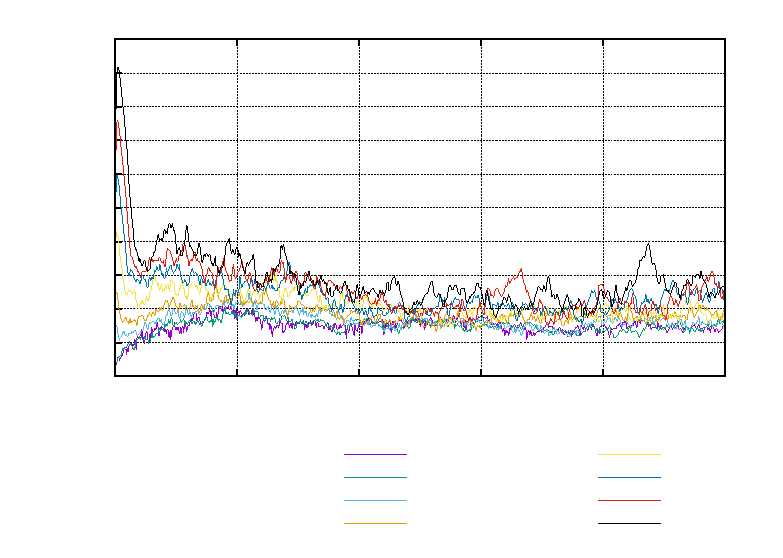
\includegraphics[width={360.00bp},height={252.00bp}]{./1000KineticComp}}%
    \gplfronttext
  \end{picture}%
\endgroup
}
        \caption{Contrainte déviatorique compression}
        \label{3000_comp}
    \end{subfigure}
    \hfill
    \begin{subfigure}[b]{0.45\textwidth}
        \centering
        \scalebox{0.5}{% GNUPLOT: LaTeX picture with Postscript
\begingroup
  \makeatletter
  \providecommand\color[2][]{%
    \GenericError{(gnuplot) \space\space\space\@spaces}{%
      Package color not loaded in conjunction with
      terminal option `colourtext'%
    }{See the gnuplot documentation for explanation.%
    }{Either use 'blacktext' in gnuplot or load the package
      color.sty in LaTeX.}%
    \renewcommand\color[2][]{}%
  }%
  \providecommand\includegraphics[2][]{%
    \GenericError{(gnuplot) \space\space\space\@spaces}{%
      Package graphicx or graphics not loaded%
    }{See the gnuplot documentation for explanation.%
    }{The gnuplot epslatex terminal needs graphicx.sty or graphics.sty.}%
    \renewcommand\includegraphics[2][]{}%
  }%
  \providecommand\rotatebox[2]{#2}%
  \@ifundefined{ifGPcolor}{%
    \newif\ifGPcolor
    \GPcolortrue
  }{}%
  \@ifundefined{ifGPblacktext}{%
    \newif\ifGPblacktext
    \GPblacktextfalse
  }{}%
  % define a \g@addto@macro without @ in the name:
  \let\gplgaddtomacro\g@addto@macro
  % define empty templates for all commands taking text:
  \gdef\gplbacktext{}%
  \gdef\gplfronttext{}%
  \makeatother
  \ifGPblacktext
    % no textcolor at all
    \def\colorrgb#1{}%
    \def\colorgray#1{}%
  \else
    % gray or color?
    \ifGPcolor
      \def\colorrgb#1{\color[rgb]{#1}}%
      \def\colorgray#1{\color[gray]{#1}}%
      \expandafter\def\csname LTw\endcsname{\color{white}}%
      \expandafter\def\csname LTb\endcsname{\color{black}}%
      \expandafter\def\csname LTa\endcsname{\color{black}}%
      \expandafter\def\csname LT0\endcsname{\color[rgb]{1,0,0}}%
      \expandafter\def\csname LT1\endcsname{\color[rgb]{0,1,0}}%
      \expandafter\def\csname LT2\endcsname{\color[rgb]{0,0,1}}%
      \expandafter\def\csname LT3\endcsname{\color[rgb]{1,0,1}}%
      \expandafter\def\csname LT4\endcsname{\color[rgb]{0,1,1}}%
      \expandafter\def\csname LT5\endcsname{\color[rgb]{1,1,0}}%
      \expandafter\def\csname LT6\endcsname{\color[rgb]{0,0,0}}%
      \expandafter\def\csname LT7\endcsname{\color[rgb]{1,0.3,0}}%
      \expandafter\def\csname LT8\endcsname{\color[rgb]{0.5,0.5,0.5}}%
    \else
      % gray
      \def\colorrgb#1{\color{black}}%
      \def\colorgray#1{\color[gray]{#1}}%
      \expandafter\def\csname LTw\endcsname{\color{white}}%
      \expandafter\def\csname LTb\endcsname{\color{black}}%
      \expandafter\def\csname LTa\endcsname{\color{black}}%
      \expandafter\def\csname LT0\endcsname{\color{black}}%
      \expandafter\def\csname LT1\endcsname{\color{black}}%
      \expandafter\def\csname LT2\endcsname{\color{black}}%
      \expandafter\def\csname LT3\endcsname{\color{black}}%
      \expandafter\def\csname LT4\endcsname{\color{black}}%
      \expandafter\def\csname LT5\endcsname{\color{black}}%
      \expandafter\def\csname LT6\endcsname{\color{black}}%
      \expandafter\def\csname LT7\endcsname{\color{black}}%
      \expandafter\def\csname LT8\endcsname{\color{black}}%
    \fi
  \fi
    \setlength{\unitlength}{0.0500bp}%
    \ifx\gptboxheight\undefined%
      \newlength{\gptboxheight}%
      \newlength{\gptboxwidth}%
      \newsavebox{\gptboxtext}%
    \fi%
    \setlength{\fboxrule}{0.5pt}%
    \setlength{\fboxsep}{1pt}%
    \definecolor{tbcol}{rgb}{1,1,1}%
\begin{picture}(7200.00,5040.00)%
    \gplgaddtomacro\gplbacktext{%
      \csname LTb\endcsname%%
      \put(814,1584){\makebox(0,0)[r]{\strut{}$-35$}}%
      \csname LTb\endcsname%%
      \put(814,2046){\makebox(0,0)[r]{\strut{}$-30$}}%
      \csname LTb\endcsname%%
      \put(814,2508){\makebox(0,0)[r]{\strut{}$-25$}}%
      \csname LTb\endcsname%%
      \put(814,2970){\makebox(0,0)[r]{\strut{}$-20$}}%
      \csname LTb\endcsname%%
      \put(814,3433){\makebox(0,0)[r]{\strut{}$-15$}}%
      \csname LTb\endcsname%%
      \put(814,3895){\makebox(0,0)[r]{\strut{}$-10$}}%
      \csname LTb\endcsname%%
      \put(814,4357){\makebox(0,0)[r]{\strut{}$-5$}}%
      \csname LTb\endcsname%%
      \put(814,4819){\makebox(0,0)[r]{\strut{}$0$}}%
      \csname LTb\endcsname%%
      \put(946,1364){\makebox(0,0){\strut{}$0$}}%
      \csname LTb\endcsname%%
      \put(2117,1364){\makebox(0,0){\strut{}$10$}}%
      \csname LTb\endcsname%%
      \put(3289,1364){\makebox(0,0){\strut{}$20$}}%
      \csname LTb\endcsname%%
      \put(4460,1364){\makebox(0,0){\strut{}$30$}}%
      \csname LTb\endcsname%%
      \put(5632,1364){\makebox(0,0){\strut{}$40$}}%
      \csname LTb\endcsname%%
      \put(6803,1364){\makebox(0,0){\strut{}$50$}}%
    }%
    \gplgaddtomacro\gplfronttext{%
      \csname LTb\endcsname%%
      \put(341,3201){\rotatebox{-270}{\makebox(0,0){\strut{}q (kPa)}}}%
      \put(3874,1034){\makebox(0,0){\strut{}$-\varepsilon_{yy}$ (\%)}}%
      \csname LTb\endcsname%%
      \put(3019,833){\makebox(0,0)[r]{\strut{}$I = 10^{-3}$}}%
      \csname LTb\endcsname%%
      \put(3019,613){\makebox(0,0)[r]{\strut{}$I = 10^{-2}$}}%
      \csname LTb\endcsname%%
      \put(3019,393){\makebox(0,0)[r]{\strut{}$I = 2 \times 10^{-2}$}}%
      \csname LTb\endcsname%%
      \put(3019,173){\makebox(0,0)[r]{\strut{}$I = 4 \times 10^{-2}$}}%
      \csname LTb\endcsname%%
      \put(5458,833){\makebox(0,0)[r]{\strut{}$I = 6 \times 10^{-2}$}}%
      \csname LTb\endcsname%%
      \put(5458,613){\makebox(0,0)[r]{\strut{}$I = 8 \times 10^{-2}$}}%
      \csname LTb\endcsname%%
      \put(5458,393){\makebox(0,0)[r]{\strut{}$I = 10^{-1}$}}%
    }%
    \gplbacktext
    \put(0,0){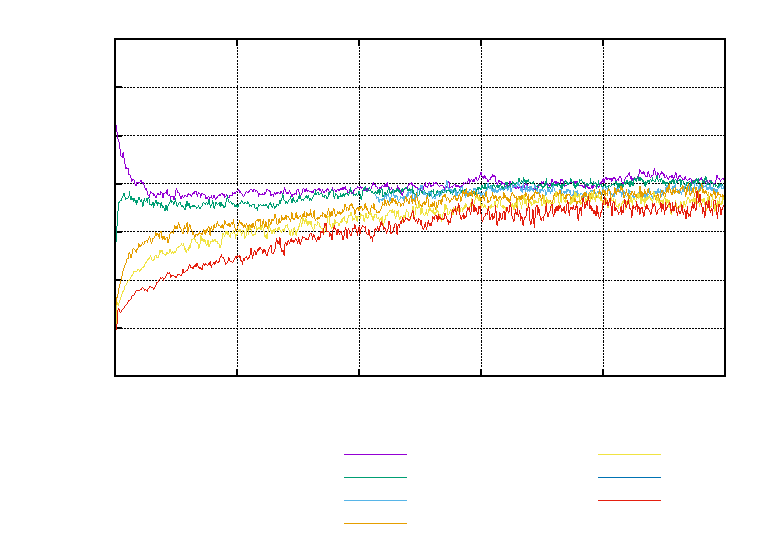
\includegraphics[width={360.00bp},height={252.00bp}]{./1000KineticExt}}%
    \gplfronttext
  \end{picture}%
\endgroup
}
        \caption{Contrainte déviatorique extension}
        \label{3000_ext}
    \end{subfigure}
    
    \begin{subfigure}[b]{0.45\textwidth}
        \centering
        \scalebox{0.5}{% GNUPLOT: LaTeX picture with Postscript
\begingroup
  \makeatletter
  \providecommand\color[2][]{%
    \GenericError{(gnuplot) \space\space\space\@spaces}{%
      Package color not loaded in conjunction with
      terminal option `colourtext'%
    }{See the gnuplot documentation for explanation.%
    }{Either use 'blacktext' in gnuplot or load the package
      color.sty in LaTeX.}%
    \renewcommand\color[2][]{}%
  }%
  \providecommand\includegraphics[2][]{%
    \GenericError{(gnuplot) \space\space\space\@spaces}{%
      Package graphicx or graphics not loaded%
    }{See the gnuplot documentation for explanation.%
    }{The gnuplot epslatex terminal needs graphicx.sty or graphics.sty.}%
    \renewcommand\includegraphics[2][]{}%
  }%
  \providecommand\rotatebox[2]{#2}%
  \@ifundefined{ifGPcolor}{%
    \newif\ifGPcolor
    \GPcolortrue
  }{}%
  \@ifundefined{ifGPblacktext}{%
    \newif\ifGPblacktext
    \GPblacktextfalse
  }{}%
  % define a \g@addto@macro without @ in the name:
  \let\gplgaddtomacro\g@addto@macro
  % define empty templates for all commands taking text:
  \gdef\gplbacktext{}%
  \gdef\gplfronttext{}%
  \makeatother
  \ifGPblacktext
    % no textcolor at all
    \def\colorrgb#1{}%
    \def\colorgray#1{}%
  \else
    % gray or color?
    \ifGPcolor
      \def\colorrgb#1{\color[rgb]{#1}}%
      \def\colorgray#1{\color[gray]{#1}}%
      \expandafter\def\csname LTw\endcsname{\color{white}}%
      \expandafter\def\csname LTb\endcsname{\color{black}}%
      \expandafter\def\csname LTa\endcsname{\color{black}}%
      \expandafter\def\csname LT0\endcsname{\color[rgb]{1,0,0}}%
      \expandafter\def\csname LT1\endcsname{\color[rgb]{0,1,0}}%
      \expandafter\def\csname LT2\endcsname{\color[rgb]{0,0,1}}%
      \expandafter\def\csname LT3\endcsname{\color[rgb]{1,0,1}}%
      \expandafter\def\csname LT4\endcsname{\color[rgb]{0,1,1}}%
      \expandafter\def\csname LT5\endcsname{\color[rgb]{1,1,0}}%
      \expandafter\def\csname LT6\endcsname{\color[rgb]{0,0,0}}%
      \expandafter\def\csname LT7\endcsname{\color[rgb]{1,0.3,0}}%
      \expandafter\def\csname LT8\endcsname{\color[rgb]{0.5,0.5,0.5}}%
    \else
      % gray
      \def\colorrgb#1{\color{black}}%
      \def\colorgray#1{\color[gray]{#1}}%
      \expandafter\def\csname LTw\endcsname{\color{white}}%
      \expandafter\def\csname LTb\endcsname{\color{black}}%
      \expandafter\def\csname LTa\endcsname{\color{black}}%
      \expandafter\def\csname LT0\endcsname{\color{black}}%
      \expandafter\def\csname LT1\endcsname{\color{black}}%
      \expandafter\def\csname LT2\endcsname{\color{black}}%
      \expandafter\def\csname LT3\endcsname{\color{black}}%
      \expandafter\def\csname LT4\endcsname{\color{black}}%
      \expandafter\def\csname LT5\endcsname{\color{black}}%
      \expandafter\def\csname LT6\endcsname{\color{black}}%
      \expandafter\def\csname LT7\endcsname{\color{black}}%
      \expandafter\def\csname LT8\endcsname{\color{black}}%
    \fi
  \fi
    \setlength{\unitlength}{0.0500bp}%
    \ifx\gptboxheight\undefined%
      \newlength{\gptboxheight}%
      \newlength{\gptboxwidth}%
      \newsavebox{\gptboxtext}%
    \fi%
    \setlength{\fboxrule}{0.5pt}%
    \setlength{\fboxsep}{1pt}%
    \definecolor{tbcol}{rgb}{1,1,1}%
\begin{picture}(9070.00,9070.00)%
    \gplgaddtomacro\gplbacktext{%
      \csname LTb\endcsname%%
      \put(814,1466){\makebox(0,0)[r]{\strut{}$-40$}}%
      \put(814,2239){\makebox(0,0)[r]{\strut{}$-30$}}%
      \put(814,3011){\makebox(0,0)[r]{\strut{}$-20$}}%
      \put(814,3784){\makebox(0,0)[r]{\strut{}$-10$}}%
      \put(814,4557){\makebox(0,0)[r]{\strut{}$0$}}%
      \put(814,5329){\makebox(0,0)[r]{\strut{}$10$}}%
      \put(814,6102){\makebox(0,0)[r]{\strut{}$20$}}%
      \put(814,6874){\makebox(0,0)[r]{\strut{}$30$}}%
      \put(814,7647){\makebox(0,0)[r]{\strut{}$40$}}%
      \put(946,4274){\makebox(0,0){\strut{} }}%
      \put(2491,4274){\makebox(0,0){\strut{}$20$}}%
      \put(4037,4274){\makebox(0,0){\strut{}$40$}}%
      \put(5582,4274){\makebox(0,0){\strut{}$60$}}%
      \put(7128,4274){\makebox(0,0){\strut{}$80$}}%
    }%
    \gplgaddtomacro\gplfronttext{%
      \csname LTb\endcsname%%
      \put(209,4556){\rotatebox{-270}{\makebox(0,0){\strut{}$\tau$ (kPa)}}}%
      \put(8505,4436){\makebox(0,0){\strut{}$\sigma_n$ (kPa)}}%
      \csname LTb\endcsname%%
      \put(6226,2959){\makebox(0,0)[r]{\strut{}$I = 10^{-3}: \varphi = 18.99^{\circ}, c = 0.09$ kPa}}%
      \csname LTb\endcsname%%
      \put(6226,2739){\makebox(0,0)[r]{\strut{}$I = 10^{-2}: \varphi = 20.60^{\circ}, c = -0.15$ kPa}}%
      \csname LTb\endcsname%%
      \put(6226,2519){\makebox(0,0)[r]{\strut{}$I = 2 \times 10^{-2}: \varphi = 25.00^{\circ}, c = -1.68$ kPa}}%
      \csname LTb\endcsname%%
      \put(6226,2299){\makebox(0,0)[r]{\strut{}$I = 4 \times 10^{-2}: \varphi = 25.59^{\circ}, c = -1.54$ kPa}}%
      \csname LTb\endcsname%%
      \put(6226,2079){\makebox(0,0)[r]{\strut{}$I = 6 \times 10^{-2}: \varphi = 19.04^{\circ}, c = 1.10$ kPa}}%
      \csname LTb\endcsname%%
      \put(6226,1859){\makebox(0,0)[r]{\strut{}$I = 8 \times 10^{-2}: \varphi = 25.14^{\circ}, c = -0.93$ kPa}}%
      \csname LTb\endcsname%%
      \put(6226,1639){\makebox(0,0)[r]{\strut{}$I = 10^{-1}: \varphi = 30.64^{\circ}, c = -2.17$ kPa}}%
    }%
    \gplbacktext
    \put(0,0){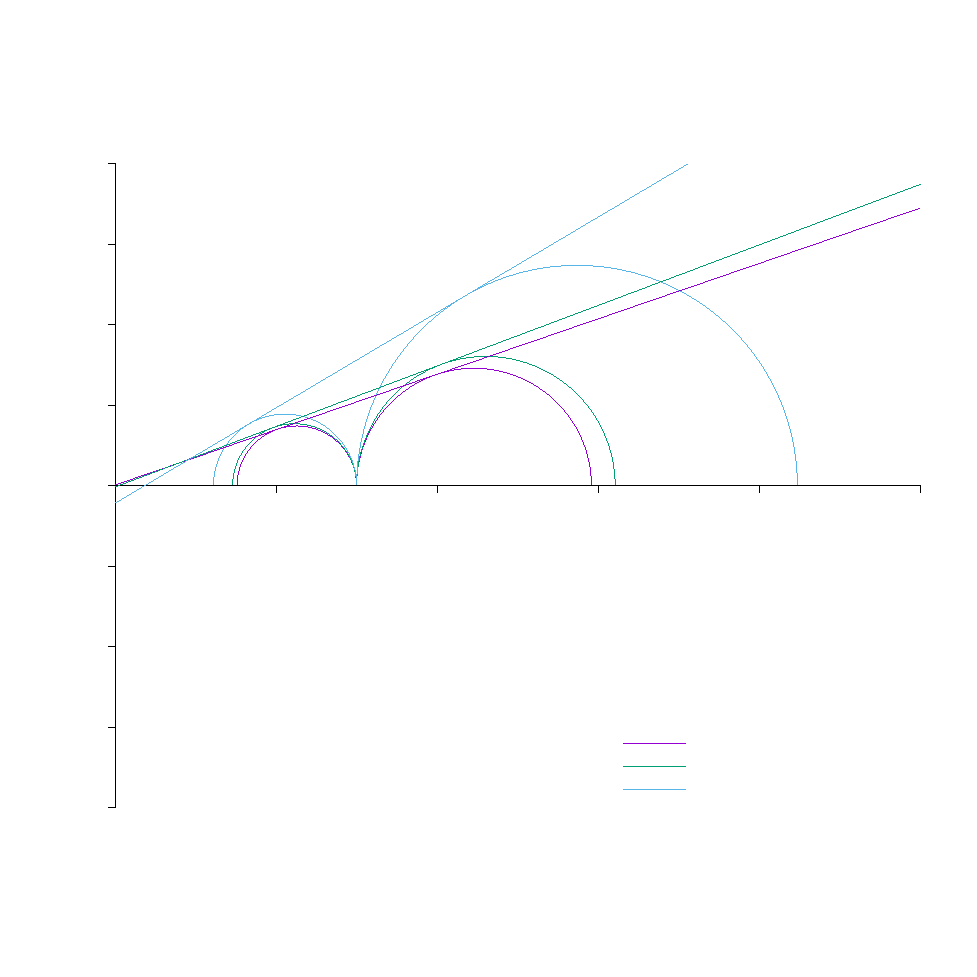
\includegraphics[width={453.50bp},height={453.50bp}]{./Cercle_3000_residuel}}%
    \gplfronttext
  \end{picture}%
\endgroup
}
        \caption{Cercle de Mohr}
        \label{300_cercle}
    \end{subfigure}
    \caption{Influence des termes cinétiques pour N=3000}
    \label{3000_Mohr}
\end{figure}

En considérant $\epsilon_{yy} = 40 \div 60\%$ comme le régime de stabilisation des contraintes (plateau d'état critique), la moyenne et l'écart-type des contraintes sont calculés, puis l'angle de frottement, ainsi que $\mu$, $\Phi$ et $e$.
Leur relation avec $I$ en échelle logarithmique est tracée selon \cref{muI, phiI}, et de même, l'indice de vide : $e = (1-\Phi)/\Phi$.
La forme des courbes est similaire à celle présentée dans \citep{da2005rheophysics}.
Les erreurs sont négligeables, comme on peut l'observer par la faible dispersion sur l'axe des ordonnées.

\begin{table}[htbp]
\centering
\small
\begin{tabular}{@{}lllllll@{}}
\toprule
\textbf{I} & $\boldsymbol{\mu}$ & $\boldsymbol{s_{\mu}}$(\%) & $\boldsymbol{\Phi}$ & $\boldsymbol{s_{\Phi}}$(\%) & $\boldsymbol{e}$ & $\boldsymbol{s_{e}}$(\%) \\
\midrule
$10^{-3}$ & 0.338 & 2.367 & 0.595 & 0.168 & 0.680 & 0.294 \\
$10^{-2}$ & 0.360 & 4.444 & 0.590 & 0.169 & 0.695 & 0.288 \\
$2 \times 10^{-2}$ & 0.406 & 4.926 & 0.583 & 0.172 & 0.714 & 0.280 \\
$4 \times 10^{-2}$ & 0.444 & 4.054 & 0.572 & 0.175 & 0.748 & 0.401 \\
$8 \times 10^{-2}$ & 0.504 & 4.365 & 0.556 & 0.180 & 0.799 & 0.375 \\
$10^{-1}$ & 0.530 & 5.283 & 0.547 & 0.366 & 0.830 & 0.843 \\
\bottomrule
\end{tabular}
\caption{Valeurs moyennes et écarts-types $\boldsymbol{s}$ de $\mu$, $\Phi$ et $e$ en fonction du nombre d'inertie pour N=3000}
\label{table_rheologie_stats}
\end{table}
% Table des valeurs moyennes et écarts-types de $\mu$, $\Phi$ et $e$ en fonction du nombre d'inertie pour N=3000

\begin{figure}[htbp]
    \centering
    \begin{subfigure}{0.9\linewidth}
        \centering
        \scalebox{0.5}{% GNUPLOT: LaTeX picture with Postscript
\begingroup
  \makeatletter
  \providecommand\color[2][]{%
    \GenericError{(gnuplot) \space\space\space\@spaces}{%
      Package color not loaded in conjunction with
      terminal option `colourtext'%
    }{See the gnuplot documentation for explanation.%
    }{Either use 'blacktext' in gnuplot or load the package
      color.sty in LaTeX.}%
    \renewcommand\color[2][]{}%
  }%
  \providecommand\includegraphics[2][]{%
    \GenericError{(gnuplot) \space\space\space\@spaces}{%
      Package graphicx or graphics not loaded%
    }{See the gnuplot documentation for explanation.%
    }{The gnuplot epslatex terminal needs graphicx.sty or graphics.sty.}%
    \renewcommand\includegraphics[2][]{}%
  }%
  \providecommand\rotatebox[2]{#2}%
  \@ifundefined{ifGPcolor}{%
    \newif\ifGPcolor
    \GPcolortrue
  }{}%
  \@ifundefined{ifGPblacktext}{%
    \newif\ifGPblacktext
    \GPblacktextfalse
  }{}%
  % define a \g@addto@macro without @ in the name:
  \let\gplgaddtomacro\g@addto@macro
  % define empty templates for all commands taking text:
  \gdef\gplbacktext{}%
  \gdef\gplfronttext{}%
  \makeatother
  \ifGPblacktext
    % no textcolor at all
    \def\colorrgb#1{}%
    \def\colorgray#1{}%
  \else
    % gray or color?
    \ifGPcolor
      \def\colorrgb#1{\color[rgb]{#1}}%
      \def\colorgray#1{\color[gray]{#1}}%
      \expandafter\def\csname LTw\endcsname{\color{white}}%
      \expandafter\def\csname LTb\endcsname{\color{black}}%
      \expandafter\def\csname LTa\endcsname{\color{black}}%
      \expandafter\def\csname LT0\endcsname{\color[rgb]{1,0,0}}%
      \expandafter\def\csname LT1\endcsname{\color[rgb]{0,1,0}}%
      \expandafter\def\csname LT2\endcsname{\color[rgb]{0,0,1}}%
      \expandafter\def\csname LT3\endcsname{\color[rgb]{1,0,1}}%
      \expandafter\def\csname LT4\endcsname{\color[rgb]{0,1,1}}%
      \expandafter\def\csname LT5\endcsname{\color[rgb]{1,1,0}}%
      \expandafter\def\csname LT6\endcsname{\color[rgb]{0,0,0}}%
      \expandafter\def\csname LT7\endcsname{\color[rgb]{1,0.3,0}}%
      \expandafter\def\csname LT8\endcsname{\color[rgb]{0.5,0.5,0.5}}%
    \else
      % gray
      \def\colorrgb#1{\color{black}}%
      \def\colorgray#1{\color[gray]{#1}}%
      \expandafter\def\csname LTw\endcsname{\color{white}}%
      \expandafter\def\csname LTb\endcsname{\color{black}}%
      \expandafter\def\csname LTa\endcsname{\color{black}}%
      \expandafter\def\csname LT0\endcsname{\color{black}}%
      \expandafter\def\csname LT1\endcsname{\color{black}}%
      \expandafter\def\csname LT2\endcsname{\color{black}}%
      \expandafter\def\csname LT3\endcsname{\color{black}}%
      \expandafter\def\csname LT4\endcsname{\color{black}}%
      \expandafter\def\csname LT5\endcsname{\color{black}}%
      \expandafter\def\csname LT6\endcsname{\color{black}}%
      \expandafter\def\csname LT7\endcsname{\color{black}}%
      \expandafter\def\csname LT8\endcsname{\color{black}}%
    \fi
  \fi
    \setlength{\unitlength}{0.0500bp}%
    \ifx\gptboxheight\undefined%
      \newlength{\gptboxheight}%
      \newlength{\gptboxwidth}%
      \newsavebox{\gptboxtext}%
    \fi%
    \setlength{\fboxrule}{0.5pt}%
    \setlength{\fboxsep}{1pt}%
    \definecolor{tbcol}{rgb}{1,1,1}%
\begin{picture}(7200.00,5040.00)%
    \gplgaddtomacro\gplbacktext{%
      \csname LTb\endcsname%%
      \put(946,704){\makebox(0,0)[r]{\strut{}$0.3$}}%
      \csname LTb\endcsname%%
      \put(946,1390){\makebox(0,0)[r]{\strut{}$0.35$}}%
      \csname LTb\endcsname%%
      \put(946,2076){\makebox(0,0)[r]{\strut{}$0.4$}}%
      \csname LTb\endcsname%%
      \put(946,2761){\makebox(0,0)[r]{\strut{}$0.45$}}%
      \csname LTb\endcsname%%
      \put(946,3447){\makebox(0,0)[r]{\strut{}$0.5$}}%
      \csname LTb\endcsname%%
      \put(946,4133){\makebox(0,0)[r]{\strut{}$0.55$}}%
      \csname LTb\endcsname%%
      \put(946,4819){\makebox(0,0)[r]{\strut{}$0.6$}}%
      \csname LTb\endcsname%%
      \put(1333,484){\makebox(0,0){\strut{}$10^{-3}$}}%
      \csname LTb\endcsname%%
      \put(3964,484){\makebox(0,0){\strut{}$10^{-2}$}}%
      \csname LTb\endcsname%%
      \put(6595,484){\makebox(0,0){\strut{}$10^{-1}$}}%
      \put(1651,3996){\makebox(0,0)[l]{\strut{}$\mu_s = 0.3317$}}%
      \put(1651,3585){\makebox(0,0)[l]{\strut{}$\mu_2 = 0.7121$}}%
      \put(1651,3173){\makebox(0,0)[l]{\strut{}$I_0 = 0.0942$}}%
    }%
    \gplgaddtomacro\gplfronttext{%
      \csname LTb\endcsname%%
      \put(209,2761){\rotatebox{-270}{\makebox(0,0){\strut{}$\mu$}}}%
      \put(3940,154){\makebox(0,0){\strut{}$I$}}%
      \csname LTb\endcsname%%
      \put(3322,4646){\makebox(0,0)[r]{\strut{}Données}}%
      \csname LTb\endcsname%%
      \put(3322,4426){\makebox(0,0)[r]{\strut{}$\mu(I)$ régression}}%
    }%
    \gplbacktext
    \put(0,0){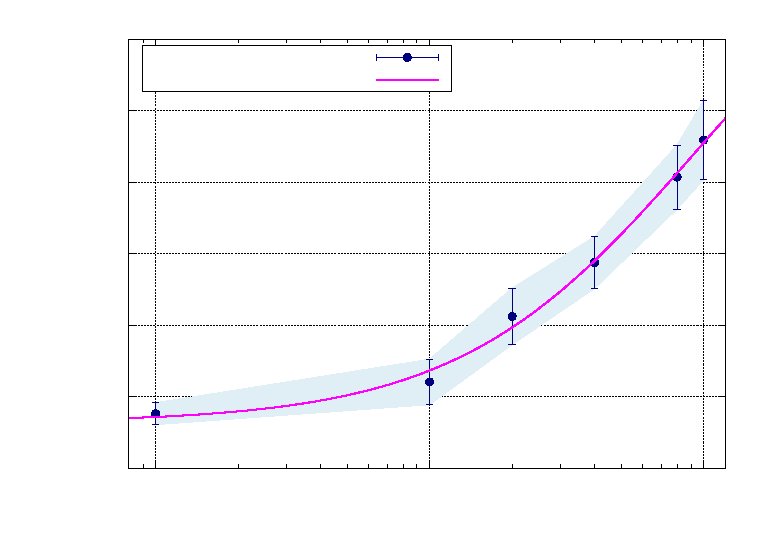
\includegraphics[width={360.00bp},height={252.00bp}]{./3000_mu_I_fit}}%
    \gplfronttext
  \end{picture}%
\endgroup
}
        \caption{$\mu(I)$}
        \label{3000_mu_I_fit}
    \end{subfigure}
    
    \begin{subfigure}{0.9\linewidth}
        \centering
        \scalebox{0.5}{% GNUPLOT: LaTeX picture with Postscript
\begingroup
  \makeatletter
  \providecommand\color[2][]{%
    \GenericError{(gnuplot) \space\space\space\@spaces}{%
      Package color not loaded in conjunction with
      terminal option `colourtext'%
    }{See the gnuplot documentation for explanation.%
    }{Either use 'blacktext' in gnuplot or load the package
      color.sty in LaTeX.}%
    \renewcommand\color[2][]{}%
  }%
  \providecommand\includegraphics[2][]{%
    \GenericError{(gnuplot) \space\space\space\@spaces}{%
      Package graphicx or graphics not loaded%
    }{See the gnuplot documentation for explanation.%
    }{The gnuplot epslatex terminal needs graphicx.sty or graphics.sty.}%
    \renewcommand\includegraphics[2][]{}%
  }%
  \providecommand\rotatebox[2]{#2}%
  \@ifundefined{ifGPcolor}{%
    \newif\ifGPcolor
    \GPcolortrue
  }{}%
  \@ifundefined{ifGPblacktext}{%
    \newif\ifGPblacktext
    \GPblacktextfalse
  }{}%
  % define a \g@addto@macro without @ in the name:
  \let\gplgaddtomacro\g@addto@macro
  % define empty templates for all commands taking text:
  \gdef\gplbacktext{}%
  \gdef\gplfronttext{}%
  \makeatother
  \ifGPblacktext
    % no textcolor at all
    \def\colorrgb#1{}%
    \def\colorgray#1{}%
  \else
    % gray or color?
    \ifGPcolor
      \def\colorrgb#1{\color[rgb]{#1}}%
      \def\colorgray#1{\color[gray]{#1}}%
      \expandafter\def\csname LTw\endcsname{\color{white}}%
      \expandafter\def\csname LTb\endcsname{\color{black}}%
      \expandafter\def\csname LTa\endcsname{\color{black}}%
      \expandafter\def\csname LT0\endcsname{\color[rgb]{1,0,0}}%
      \expandafter\def\csname LT1\endcsname{\color[rgb]{0,1,0}}%
      \expandafter\def\csname LT2\endcsname{\color[rgb]{0,0,1}}%
      \expandafter\def\csname LT3\endcsname{\color[rgb]{1,0,1}}%
      \expandafter\def\csname LT4\endcsname{\color[rgb]{0,1,1}}%
      \expandafter\def\csname LT5\endcsname{\color[rgb]{1,1,0}}%
      \expandafter\def\csname LT6\endcsname{\color[rgb]{0,0,0}}%
      \expandafter\def\csname LT7\endcsname{\color[rgb]{1,0.3,0}}%
      \expandafter\def\csname LT8\endcsname{\color[rgb]{0.5,0.5,0.5}}%
    \else
      % gray
      \def\colorrgb#1{\color{black}}%
      \def\colorgray#1{\color[gray]{#1}}%
      \expandafter\def\csname LTw\endcsname{\color{white}}%
      \expandafter\def\csname LTb\endcsname{\color{black}}%
      \expandafter\def\csname LTa\endcsname{\color{black}}%
      \expandafter\def\csname LT0\endcsname{\color{black}}%
      \expandafter\def\csname LT1\endcsname{\color{black}}%
      \expandafter\def\csname LT2\endcsname{\color{black}}%
      \expandafter\def\csname LT3\endcsname{\color{black}}%
      \expandafter\def\csname LT4\endcsname{\color{black}}%
      \expandafter\def\csname LT5\endcsname{\color{black}}%
      \expandafter\def\csname LT6\endcsname{\color{black}}%
      \expandafter\def\csname LT7\endcsname{\color{black}}%
      \expandafter\def\csname LT8\endcsname{\color{black}}%
    \fi
  \fi
    \setlength{\unitlength}{0.0500bp}%
    \ifx\gptboxheight\undefined%
      \newlength{\gptboxheight}%
      \newlength{\gptboxwidth}%
      \newsavebox{\gptboxtext}%
    \fi%
    \setlength{\fboxrule}{0.5pt}%
    \setlength{\fboxsep}{1pt}%
    \definecolor{tbcol}{rgb}{1,1,1}%
\begin{picture}(7200.00,5040.00)%
    \gplgaddtomacro\gplbacktext{%
      \csname LTb\endcsname%%
      \put(946,704){\makebox(0,0)[r]{\strut{}$0.53$}}%
      \csname LTb\endcsname%%
      \put(946,1292){\makebox(0,0)[r]{\strut{}$0.54$}}%
      \csname LTb\endcsname%%
      \put(946,1880){\makebox(0,0)[r]{\strut{}$0.55$}}%
      \csname LTb\endcsname%%
      \put(946,2468){\makebox(0,0)[r]{\strut{}$0.56$}}%
      \csname LTb\endcsname%%
      \put(946,3055){\makebox(0,0)[r]{\strut{}$0.57$}}%
      \csname LTb\endcsname%%
      \put(946,3643){\makebox(0,0)[r]{\strut{}$0.58$}}%
      \csname LTb\endcsname%%
      \put(946,4231){\makebox(0,0)[r]{\strut{}$0.59$}}%
      \csname LTb\endcsname%%
      \put(946,4819){\makebox(0,0)[r]{\strut{}$0.6$}}%
      \csname LTb\endcsname%%
      \put(1333,484){\makebox(0,0){\strut{}$10^{-3}$}}%
      \csname LTb\endcsname%%
      \put(3964,484){\makebox(0,0){\strut{}$10^{-2}$}}%
      \csname LTb\endcsname%%
      \put(6595,484){\makebox(0,0){\strut{}$10^{-1}$}}%
      \put(1651,1733){\makebox(0,0)[l]{\strut{}$\Phi_{max} = 0.5941$}}%
      \put(1651,1321){\makebox(0,0)[l]{\strut{}$b = 0.4829$}}%
    }%
    \gplgaddtomacro\gplfronttext{%
      \csname LTb\endcsname%%
      \put(209,2761){\rotatebox{-270}{\makebox(0,0){\strut{}$\phi$}}}%
      \put(3940,154){\makebox(0,0){\strut{}$I$}}%
      \csname LTb\endcsname%%
      \put(3322,1097){\makebox(0,0)[r]{\strut{}Données}}%
      \csname LTb\endcsname%%
      \put(3322,877){\makebox(0,0)[r]{\strut{}$\Phi(I)$ régression}}%
    }%
    \gplbacktext
    \put(0,0){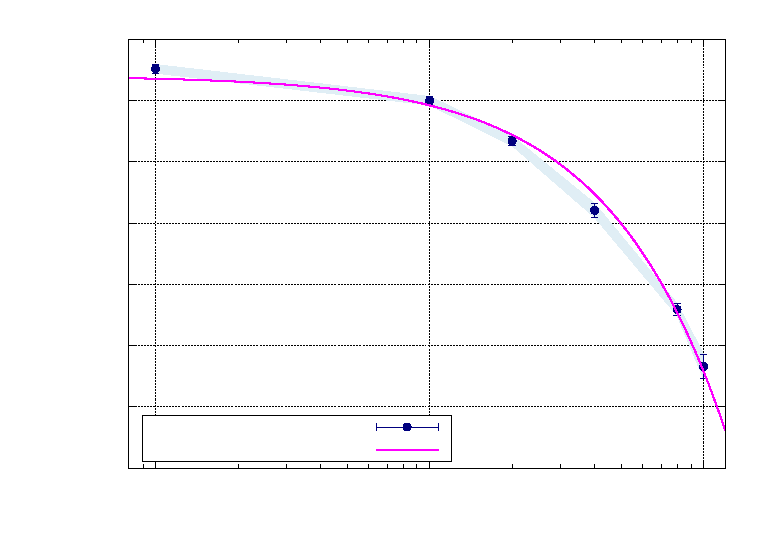
\includegraphics[width={360.00bp},height={252.00bp}]{./3000_phi_I_fit}}%
    \gplfronttext
  \end{picture}%
\endgroup
}
        \caption{$\Phi(I)$}
        \label{3000_phi_I_fit}
    \end{subfigure}
    
    \begin{subfigure}{0.9\linewidth}
        \centering
        \scalebox{0.5}{% GNUPLOT: LaTeX picture with Postscript
\begingroup
  \makeatletter
  \providecommand\color[2][]{%
    \GenericError{(gnuplot) \space\space\space\@spaces}{%
      Package color not loaded in conjunction with
      terminal option `colourtext'%
    }{See the gnuplot documentation for explanation.%
    }{Either use 'blacktext' in gnuplot or load the package
      color.sty in LaTeX.}%
    \renewcommand\color[2][]{}%
  }%
  \providecommand\includegraphics[2][]{%
    \GenericError{(gnuplot) \space\space\space\@spaces}{%
      Package graphicx or graphics not loaded%
    }{See the gnuplot documentation for explanation.%
    }{The gnuplot epslatex terminal needs graphicx.sty or graphics.sty.}%
    \renewcommand\includegraphics[2][]{}%
  }%
  \providecommand\rotatebox[2]{#2}%
  \@ifundefined{ifGPcolor}{%
    \newif\ifGPcolor
    \GPcolortrue
  }{}%
  \@ifundefined{ifGPblacktext}{%
    \newif\ifGPblacktext
    \GPblacktextfalse
  }{}%
  % define a \g@addto@macro without @ in the name:
  \let\gplgaddtomacro\g@addto@macro
  % define empty templates for all commands taking text:
  \gdef\gplbacktext{}%
  \gdef\gplfronttext{}%
  \makeatother
  \ifGPblacktext
    % no textcolor at all
    \def\colorrgb#1{}%
    \def\colorgray#1{}%
  \else
    % gray or color?
    \ifGPcolor
      \def\colorrgb#1{\color[rgb]{#1}}%
      \def\colorgray#1{\color[gray]{#1}}%
      \expandafter\def\csname LTw\endcsname{\color{white}}%
      \expandafter\def\csname LTb\endcsname{\color{black}}%
      \expandafter\def\csname LTa\endcsname{\color{black}}%
      \expandafter\def\csname LT0\endcsname{\color[rgb]{1,0,0}}%
      \expandafter\def\csname LT1\endcsname{\color[rgb]{0,1,0}}%
      \expandafter\def\csname LT2\endcsname{\color[rgb]{0,0,1}}%
      \expandafter\def\csname LT3\endcsname{\color[rgb]{1,0,1}}%
      \expandafter\def\csname LT4\endcsname{\color[rgb]{0,1,1}}%
      \expandafter\def\csname LT5\endcsname{\color[rgb]{1,1,0}}%
      \expandafter\def\csname LT6\endcsname{\color[rgb]{0,0,0}}%
      \expandafter\def\csname LT7\endcsname{\color[rgb]{1,0.3,0}}%
      \expandafter\def\csname LT8\endcsname{\color[rgb]{0.5,0.5,0.5}}%
    \else
      % gray
      \def\colorrgb#1{\color{black}}%
      \def\colorgray#1{\color[gray]{#1}}%
      \expandafter\def\csname LTw\endcsname{\color{white}}%
      \expandafter\def\csname LTb\endcsname{\color{black}}%
      \expandafter\def\csname LTa\endcsname{\color{black}}%
      \expandafter\def\csname LT0\endcsname{\color{black}}%
      \expandafter\def\csname LT1\endcsname{\color{black}}%
      \expandafter\def\csname LT2\endcsname{\color{black}}%
      \expandafter\def\csname LT3\endcsname{\color{black}}%
      \expandafter\def\csname LT4\endcsname{\color{black}}%
      \expandafter\def\csname LT5\endcsname{\color{black}}%
      \expandafter\def\csname LT6\endcsname{\color{black}}%
      \expandafter\def\csname LT7\endcsname{\color{black}}%
      \expandafter\def\csname LT8\endcsname{\color{black}}%
    \fi
  \fi
    \setlength{\unitlength}{0.0500bp}%
    \ifx\gptboxheight\undefined%
      \newlength{\gptboxheight}%
      \newlength{\gptboxwidth}%
      \newsavebox{\gptboxtext}%
    \fi%
    \setlength{\fboxrule}{0.5pt}%
    \setlength{\fboxsep}{1pt}%
    \definecolor{tbcol}{rgb}{1,1,1}%
\begin{picture}(7200.00,5040.00)%
    \gplgaddtomacro\gplbacktext{%
      \csname LTb\endcsname%%
      \put(946,704){\makebox(0,0)[r]{\strut{}$0.66$}}%
      \csname LTb\endcsname%%
      \put(946,1078){\makebox(0,0)[r]{\strut{}$0.68$}}%
      \csname LTb\endcsname%%
      \put(946,1452){\makebox(0,0)[r]{\strut{}$0.7$}}%
      \csname LTb\endcsname%%
      \put(946,1826){\makebox(0,0)[r]{\strut{}$0.72$}}%
      \csname LTb\endcsname%%
      \put(946,2200){\makebox(0,0)[r]{\strut{}$0.74$}}%
      \csname LTb\endcsname%%
      \put(946,2574){\makebox(0,0)[r]{\strut{}$0.76$}}%
      \csname LTb\endcsname%%
      \put(946,2949){\makebox(0,0)[r]{\strut{}$0.78$}}%
      \csname LTb\endcsname%%
      \put(946,3323){\makebox(0,0)[r]{\strut{}$0.8$}}%
      \csname LTb\endcsname%%
      \put(946,3697){\makebox(0,0)[r]{\strut{}$0.82$}}%
      \csname LTb\endcsname%%
      \put(946,4071){\makebox(0,0)[r]{\strut{}$0.84$}}%
      \csname LTb\endcsname%%
      \put(946,4445){\makebox(0,0)[r]{\strut{}$0.86$}}%
      \csname LTb\endcsname%%
      \put(946,4819){\makebox(0,0)[r]{\strut{}$0.88$}}%
      \csname LTb\endcsname%%
      \put(1333,484){\makebox(0,0){\strut{}$10^{-3}$}}%
      \csname LTb\endcsname%%
      \put(3964,484){\makebox(0,0){\strut{}$10^{-2}$}}%
      \csname LTb\endcsname%%
      \put(6595,484){\makebox(0,0){\strut{}$10^{-1}$}}%
    }%
    \gplgaddtomacro\gplfronttext{%
      \csname LTb\endcsname%%
      \put(209,2761){\rotatebox{-270}{\makebox(0,0){\strut{}$e$}}}%
      \put(3940,154){\makebox(0,0){\strut{}$I$}}%
      \csname LTb\endcsname%%
      \put(3322,4646){\makebox(0,0)[r]{\strut{}Données}}%
      \csname LTb\endcsname%%
      \put(3322,4426){\makebox(0,0)[r]{\strut{}e(I) régression}}%
    }%
    \gplbacktext
    \put(0,0){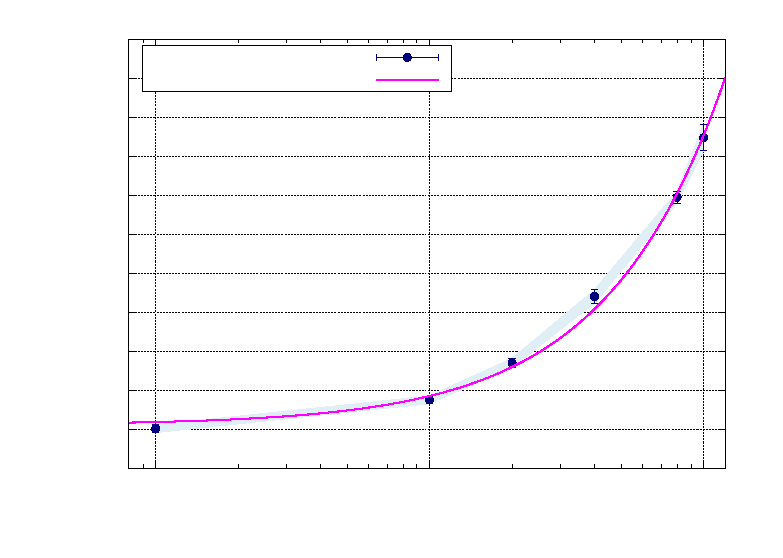
\includegraphics[width={360.00bp},height={252.00bp}]{./3000_e_I_plot}}%
    \gplfronttext
  \end{picture}%
\endgroup
}
        \caption{$e(I)$}
        \label{3000_e_I_fit}
    \end{subfigure}
    \caption{Rhéologies $\mu(I)$, $\Phi(I)$ et $e(I)$ quand $\epsilon_{yy} = 40 \div 60\%$ pour N=3000}
    \label{rheologies_3000}
\end{figure}


\begin{figure}[htbp]
    \centering
    \begin{subfigure}{0.9\linewidth}
        \centering
        \scalebox{0.5}{% GNUPLOT: LaTeX picture with Postscript
\begingroup
  \makeatletter
  \providecommand\color[2][]{%
    \GenericError{(gnuplot) \space\space\space\@spaces}{%
      Package color not loaded in conjunction with
      terminal option `colourtext'%
    }{See the gnuplot documentation for explanation.%
    }{Either use 'blacktext' in gnuplot or load the package
      color.sty in LaTeX.}%
    \renewcommand\color[2][]{}%
  }%
  \providecommand\includegraphics[2][]{%
    \GenericError{(gnuplot) \space\space\space\@spaces}{%
      Package graphicx or graphics not loaded%
    }{See the gnuplot documentation for explanation.%
    }{The gnuplot epslatex terminal needs graphicx.sty or graphics.sty.}%
    \renewcommand\includegraphics[2][]{}%
  }%
  \providecommand\rotatebox[2]{#2}%
  \@ifundefined{ifGPcolor}{%
    \newif\ifGPcolor
    \GPcolortrue
  }{}%
  \@ifundefined{ifGPblacktext}{%
    \newif\ifGPblacktext
    \GPblacktextfalse
  }{}%
  % define a \g@addto@macro without @ in the name:
  \let\gplgaddtomacro\g@addto@macro
  % define empty templates for all commands taking text:
  \gdef\gplbacktext{}%
  \gdef\gplfronttext{}%
  \makeatother
  \ifGPblacktext
    % no textcolor at all
    \def\colorrgb#1{}%
    \def\colorgray#1{}%
  \else
    % gray or color?
    \ifGPcolor
      \def\colorrgb#1{\color[rgb]{#1}}%
      \def\colorgray#1{\color[gray]{#1}}%
      \expandafter\def\csname LTw\endcsname{\color{white}}%
      \expandafter\def\csname LTb\endcsname{\color{black}}%
      \expandafter\def\csname LTa\endcsname{\color{black}}%
      \expandafter\def\csname LT0\endcsname{\color[rgb]{1,0,0}}%
      \expandafter\def\csname LT1\endcsname{\color[rgb]{0,1,0}}%
      \expandafter\def\csname LT2\endcsname{\color[rgb]{0,0,1}}%
      \expandafter\def\csname LT3\endcsname{\color[rgb]{1,0,1}}%
      \expandafter\def\csname LT4\endcsname{\color[rgb]{0,1,1}}%
      \expandafter\def\csname LT5\endcsname{\color[rgb]{1,1,0}}%
      \expandafter\def\csname LT6\endcsname{\color[rgb]{0,0,0}}%
      \expandafter\def\csname LT7\endcsname{\color[rgb]{1,0.3,0}}%
      \expandafter\def\csname LT8\endcsname{\color[rgb]{0.5,0.5,0.5}}%
    \else
      % gray
      \def\colorrgb#1{\color{black}}%
      \def\colorgray#1{\color[gray]{#1}}%
      \expandafter\def\csname LTw\endcsname{\color{white}}%
      \expandafter\def\csname LTb\endcsname{\color{black}}%
      \expandafter\def\csname LTa\endcsname{\color{black}}%
      \expandafter\def\csname LT0\endcsname{\color{black}}%
      \expandafter\def\csname LT1\endcsname{\color{black}}%
      \expandafter\def\csname LT2\endcsname{\color{black}}%
      \expandafter\def\csname LT3\endcsname{\color{black}}%
      \expandafter\def\csname LT4\endcsname{\color{black}}%
      \expandafter\def\csname LT5\endcsname{\color{black}}%
      \expandafter\def\csname LT6\endcsname{\color{black}}%
      \expandafter\def\csname LT7\endcsname{\color{black}}%
      \expandafter\def\csname LT8\endcsname{\color{black}}%
    \fi
  \fi
    \setlength{\unitlength}{0.0500bp}%
    \ifx\gptboxheight\undefined%
      \newlength{\gptboxheight}%
      \newlength{\gptboxwidth}%
      \newsavebox{\gptboxtext}%
    \fi%
    \setlength{\fboxrule}{0.5pt}%
    \setlength{\fboxsep}{1pt}%
    \definecolor{tbcol}{rgb}{1,1,1}%
\begin{picture}(7200.00,5040.00)%
    \gplgaddtomacro\gplbacktext{%
      \csname LTb\endcsname%%
      \put(946,704){\makebox(0,0)[r]{\strut{}$0.3$}}%
      \csname LTb\endcsname%%
      \put(946,1292){\makebox(0,0)[r]{\strut{}$0.35$}}%
      \csname LTb\endcsname%%
      \put(946,1880){\makebox(0,0)[r]{\strut{}$0.4$}}%
      \csname LTb\endcsname%%
      \put(946,2468){\makebox(0,0)[r]{\strut{}$0.45$}}%
      \csname LTb\endcsname%%
      \put(946,3055){\makebox(0,0)[r]{\strut{}$0.5$}}%
      \csname LTb\endcsname%%
      \put(946,3643){\makebox(0,0)[r]{\strut{}$0.55$}}%
      \csname LTb\endcsname%%
      \put(946,4231){\makebox(0,0)[r]{\strut{}$0.6$}}%
      \csname LTb\endcsname%%
      \put(946,4819){\makebox(0,0)[r]{\strut{}$0.65$}}%
      \csname LTb\endcsname%%
      \put(1333,484){\makebox(0,0){\strut{}$10^{-3}$}}%
      \csname LTb\endcsname%%
      \put(3964,484){\makebox(0,0){\strut{}$10^{-2}$}}%
      \csname LTb\endcsname%%
      \put(6595,484){\makebox(0,0){\strut{}$10^{-1}$}}%
      \put(1651,3996){\makebox(0,0)[l]{\strut{}$\mu_s = 0.3505$}}%
      \put(1651,3585){\makebox(0,0)[l]{\strut{}$\mu_2 = 2.5598$}}%
      \put(1651,3173){\makebox(0,0)[l]{\strut{}$I_0 = 1.0000$}}%
    }%
    \gplgaddtomacro\gplfronttext{%
      \csname LTb\endcsname%%
      \put(209,2761){\rotatebox{-270}{\makebox(0,0){\strut{}$\mu$}}}%
      \put(3940,154){\makebox(0,0){\strut{}$I$}}%
      \csname LTb\endcsname%%
      \put(3322,4646){\makebox(0,0)[r]{\strut{}Données}}%
      \csname LTb\endcsname%%
      \put(3322,4426){\makebox(0,0)[r]{\strut{}$\mu(I)$ régression}}%
    }%
    \gplbacktext
    \put(0,0){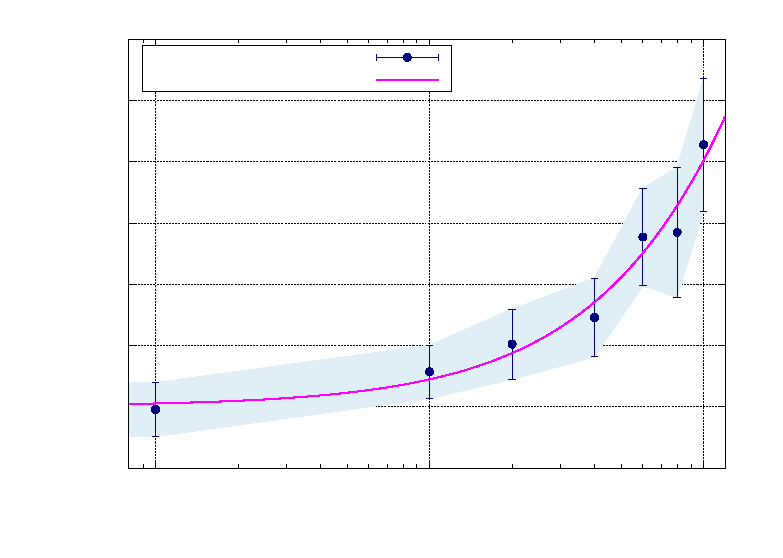
\includegraphics[width={360.00bp},height={252.00bp}]{./1000_mu_I_fit}}%
    \gplfronttext
  \end{picture}%
\endgroup
}
        \caption{$\mu(I)$}
        \label{1000_mu_I_fit}
    \end{subfigure}
    
    \begin{subfigure}{0.9\linewidth}
        \centering
        \scalebox{0.5}{% GNUPLOT: LaTeX picture with Postscript
\begingroup
  \makeatletter
  \providecommand\color[2][]{%
    \GenericError{(gnuplot) \space\space\space\@spaces}{%
      Package color not loaded in conjunction with
      terminal option `colourtext'%
    }{See the gnuplot documentation for explanation.%
    }{Either use 'blacktext' in gnuplot or load the package
      color.sty in LaTeX.}%
    \renewcommand\color[2][]{}%
  }%
  \providecommand\includegraphics[2][]{%
    \GenericError{(gnuplot) \space\space\space\@spaces}{%
      Package graphicx or graphics not loaded%
    }{See the gnuplot documentation for explanation.%
    }{The gnuplot epslatex terminal needs graphicx.sty or graphics.sty.}%
    \renewcommand\includegraphics[2][]{}%
  }%
  \providecommand\rotatebox[2]{#2}%
  \@ifundefined{ifGPcolor}{%
    \newif\ifGPcolor
    \GPcolortrue
  }{}%
  \@ifundefined{ifGPblacktext}{%
    \newif\ifGPblacktext
    \GPblacktextfalse
  }{}%
  % define a \g@addto@macro without @ in the name:
  \let\gplgaddtomacro\g@addto@macro
  % define empty templates for all commands taking text:
  \gdef\gplbacktext{}%
  \gdef\gplfronttext{}%
  \makeatother
  \ifGPblacktext
    % no textcolor at all
    \def\colorrgb#1{}%
    \def\colorgray#1{}%
  \else
    % gray or color?
    \ifGPcolor
      \def\colorrgb#1{\color[rgb]{#1}}%
      \def\colorgray#1{\color[gray]{#1}}%
      \expandafter\def\csname LTw\endcsname{\color{white}}%
      \expandafter\def\csname LTb\endcsname{\color{black}}%
      \expandafter\def\csname LTa\endcsname{\color{black}}%
      \expandafter\def\csname LT0\endcsname{\color[rgb]{1,0,0}}%
      \expandafter\def\csname LT1\endcsname{\color[rgb]{0,1,0}}%
      \expandafter\def\csname LT2\endcsname{\color[rgb]{0,0,1}}%
      \expandafter\def\csname LT3\endcsname{\color[rgb]{1,0,1}}%
      \expandafter\def\csname LT4\endcsname{\color[rgb]{0,1,1}}%
      \expandafter\def\csname LT5\endcsname{\color[rgb]{1,1,0}}%
      \expandafter\def\csname LT6\endcsname{\color[rgb]{0,0,0}}%
      \expandafter\def\csname LT7\endcsname{\color[rgb]{1,0.3,0}}%
      \expandafter\def\csname LT8\endcsname{\color[rgb]{0.5,0.5,0.5}}%
    \else
      % gray
      \def\colorrgb#1{\color{black}}%
      \def\colorgray#1{\color[gray]{#1}}%
      \expandafter\def\csname LTw\endcsname{\color{white}}%
      \expandafter\def\csname LTb\endcsname{\color{black}}%
      \expandafter\def\csname LTa\endcsname{\color{black}}%
      \expandafter\def\csname LT0\endcsname{\color{black}}%
      \expandafter\def\csname LT1\endcsname{\color{black}}%
      \expandafter\def\csname LT2\endcsname{\color{black}}%
      \expandafter\def\csname LT3\endcsname{\color{black}}%
      \expandafter\def\csname LT4\endcsname{\color{black}}%
      \expandafter\def\csname LT5\endcsname{\color{black}}%
      \expandafter\def\csname LT6\endcsname{\color{black}}%
      \expandafter\def\csname LT7\endcsname{\color{black}}%
      \expandafter\def\csname LT8\endcsname{\color{black}}%
    \fi
  \fi
    \setlength{\unitlength}{0.0500bp}%
    \ifx\gptboxheight\undefined%
      \newlength{\gptboxheight}%
      \newlength{\gptboxwidth}%
      \newsavebox{\gptboxtext}%
    \fi%
    \setlength{\fboxrule}{0.5pt}%
    \setlength{\fboxsep}{1pt}%
    \definecolor{tbcol}{rgb}{1,1,1}%
\begin{picture}(7200.00,5040.00)%
    \gplgaddtomacro\gplbacktext{%
      \csname LTb\endcsname%%
      \put(946,704){\makebox(0,0)[r]{\strut{}$0.53$}}%
      \csname LTb\endcsname%%
      \put(946,1292){\makebox(0,0)[r]{\strut{}$0.54$}}%
      \csname LTb\endcsname%%
      \put(946,1880){\makebox(0,0)[r]{\strut{}$0.55$}}%
      \csname LTb\endcsname%%
      \put(946,2468){\makebox(0,0)[r]{\strut{}$0.56$}}%
      \csname LTb\endcsname%%
      \put(946,3055){\makebox(0,0)[r]{\strut{}$0.57$}}%
      \csname LTb\endcsname%%
      \put(946,3643){\makebox(0,0)[r]{\strut{}$0.58$}}%
      \csname LTb\endcsname%%
      \put(946,4231){\makebox(0,0)[r]{\strut{}$0.59$}}%
      \csname LTb\endcsname%%
      \put(946,4819){\makebox(0,0)[r]{\strut{}$0.6$}}%
      \csname LTb\endcsname%%
      \put(1333,484){\makebox(0,0){\strut{}$10^{-3}$}}%
      \csname LTb\endcsname%%
      \put(3964,484){\makebox(0,0){\strut{}$10^{-2}$}}%
      \csname LTb\endcsname%%
      \put(6595,484){\makebox(0,0){\strut{}$10^{-1}$}}%
      \put(1651,1733){\makebox(0,0)[l]{\strut{}$\Phi_{max} = 0.5944$}}%
      \put(1651,1321){\makebox(0,0)[l]{\strut{}$b = 0.4551$}}%
    }%
    \gplgaddtomacro\gplfronttext{%
      \csname LTb\endcsname%%
      \put(209,2761){\rotatebox{-270}{\makebox(0,0){\strut{}$\Phi$}}}%
      \put(3940,154){\makebox(0,0){\strut{}$I$}}%
      \csname LTb\endcsname%%
      \put(3322,1097){\makebox(0,0)[r]{\strut{}Données}}%
      \csname LTb\endcsname%%
      \put(3322,877){\makebox(0,0)[r]{\strut{}$\Phi(I)$ régression}}%
    }%
    \gplbacktext
    \put(0,0){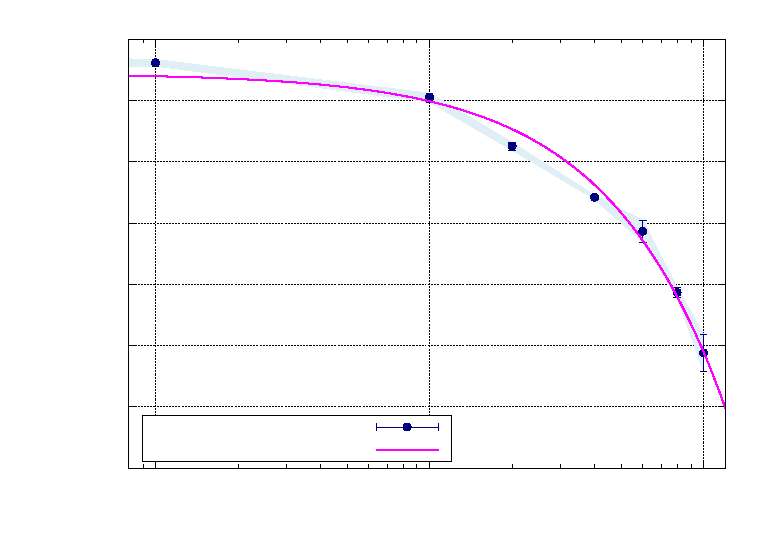
\includegraphics[width={360.00bp},height={252.00bp}]{./1000_phi_I_fit}}%
    \gplfronttext
  \end{picture}%
\endgroup
}
        \caption{$\Phi(I)$}
        \label{1000_phi_I_fit}
    \end{subfigure}
    
    \begin{subfigure}{0.9\linewidth}
        \centering
        \scalebox{0.5}{% GNUPLOT: LaTeX picture with Postscript
\begingroup
  \makeatletter
  \providecommand\color[2][]{%
    \GenericError{(gnuplot) \space\space\space\@spaces}{%
      Package color not loaded in conjunction with
      terminal option `colourtext'%
    }{See the gnuplot documentation for explanation.%
    }{Either use 'blacktext' in gnuplot or load the package
      color.sty in LaTeX.}%
    \renewcommand\color[2][]{}%
  }%
  \providecommand\includegraphics[2][]{%
    \GenericError{(gnuplot) \space\space\space\@spaces}{%
      Package graphicx or graphics not loaded%
    }{See the gnuplot documentation for explanation.%
    }{The gnuplot epslatex terminal needs graphicx.sty or graphics.sty.}%
    \renewcommand\includegraphics[2][]{}%
  }%
  \providecommand\rotatebox[2]{#2}%
  \@ifundefined{ifGPcolor}{%
    \newif\ifGPcolor
    \GPcolortrue
  }{}%
  \@ifundefined{ifGPblacktext}{%
    \newif\ifGPblacktext
    \GPblacktextfalse
  }{}%
  % define a \g@addto@macro without @ in the name:
  \let\gplgaddtomacro\g@addto@macro
  % define empty templates for all commands taking text:
  \gdef\gplbacktext{}%
  \gdef\gplfronttext{}%
  \makeatother
  \ifGPblacktext
    % no textcolor at all
    \def\colorrgb#1{}%
    \def\colorgray#1{}%
  \else
    % gray or color?
    \ifGPcolor
      \def\colorrgb#1{\color[rgb]{#1}}%
      \def\colorgray#1{\color[gray]{#1}}%
      \expandafter\def\csname LTw\endcsname{\color{white}}%
      \expandafter\def\csname LTb\endcsname{\color{black}}%
      \expandafter\def\csname LTa\endcsname{\color{black}}%
      \expandafter\def\csname LT0\endcsname{\color[rgb]{1,0,0}}%
      \expandafter\def\csname LT1\endcsname{\color[rgb]{0,1,0}}%
      \expandafter\def\csname LT2\endcsname{\color[rgb]{0,0,1}}%
      \expandafter\def\csname LT3\endcsname{\color[rgb]{1,0,1}}%
      \expandafter\def\csname LT4\endcsname{\color[rgb]{0,1,1}}%
      \expandafter\def\csname LT5\endcsname{\color[rgb]{1,1,0}}%
      \expandafter\def\csname LT6\endcsname{\color[rgb]{0,0,0}}%
      \expandafter\def\csname LT7\endcsname{\color[rgb]{1,0.3,0}}%
      \expandafter\def\csname LT8\endcsname{\color[rgb]{0.5,0.5,0.5}}%
    \else
      % gray
      \def\colorrgb#1{\color{black}}%
      \def\colorgray#1{\color[gray]{#1}}%
      \expandafter\def\csname LTw\endcsname{\color{white}}%
      \expandafter\def\csname LTb\endcsname{\color{black}}%
      \expandafter\def\csname LTa\endcsname{\color{black}}%
      \expandafter\def\csname LT0\endcsname{\color{black}}%
      \expandafter\def\csname LT1\endcsname{\color{black}}%
      \expandafter\def\csname LT2\endcsname{\color{black}}%
      \expandafter\def\csname LT3\endcsname{\color{black}}%
      \expandafter\def\csname LT4\endcsname{\color{black}}%
      \expandafter\def\csname LT5\endcsname{\color{black}}%
      \expandafter\def\csname LT6\endcsname{\color{black}}%
      \expandafter\def\csname LT7\endcsname{\color{black}}%
      \expandafter\def\csname LT8\endcsname{\color{black}}%
    \fi
  \fi
    \setlength{\unitlength}{0.0500bp}%
    \ifx\gptboxheight\undefined%
      \newlength{\gptboxheight}%
      \newlength{\gptboxwidth}%
      \newsavebox{\gptboxtext}%
    \fi%
    \setlength{\fboxrule}{0.5pt}%
    \setlength{\fboxsep}{1pt}%
    \definecolor{tbcol}{rgb}{1,1,1}%
\begin{picture}(7200.00,5040.00)%
    \gplgaddtomacro\gplbacktext{%
      \csname LTb\endcsname%%
      \put(946,704){\makebox(0,0)[r]{\strut{}$0.66$}}%
      \csname LTb\endcsname%%
      \put(946,1116){\makebox(0,0)[r]{\strut{}$0.68$}}%
      \csname LTb\endcsname%%
      \put(946,1527){\makebox(0,0)[r]{\strut{}$0.7$}}%
      \csname LTb\endcsname%%
      \put(946,1939){\makebox(0,0)[r]{\strut{}$0.72$}}%
      \csname LTb\endcsname%%
      \put(946,2350){\makebox(0,0)[r]{\strut{}$0.74$}}%
      \csname LTb\endcsname%%
      \put(946,2762){\makebox(0,0)[r]{\strut{}$0.76$}}%
      \csname LTb\endcsname%%
      \put(946,3173){\makebox(0,0)[r]{\strut{}$0.78$}}%
      \csname LTb\endcsname%%
      \put(946,3585){\makebox(0,0)[r]{\strut{}$0.8$}}%
      \csname LTb\endcsname%%
      \put(946,3996){\makebox(0,0)[r]{\strut{}$0.82$}}%
      \csname LTb\endcsname%%
      \put(946,4408){\makebox(0,0)[r]{\strut{}$0.84$}}%
      \csname LTb\endcsname%%
      \put(946,4819){\makebox(0,0)[r]{\strut{}$0.86$}}%
      \csname LTb\endcsname%%
      \put(1333,484){\makebox(0,0){\strut{}$10^{-3}$}}%
      \csname LTb\endcsname%%
      \put(3964,484){\makebox(0,0){\strut{}$10^{-2}$}}%
      \csname LTb\endcsname%%
      \put(6595,484){\makebox(0,0){\strut{}$10^{-1}$}}%
    }%
    \gplgaddtomacro\gplfronttext{%
      \csname LTb\endcsname%%
      \put(209,2761){\rotatebox{-270}{\makebox(0,0){\strut{}$e$}}}%
      \put(3940,154){\makebox(0,0){\strut{}$I$}}%
      \csname LTb\endcsname%%
      \put(3322,4646){\makebox(0,0)[r]{\strut{}Données}}%
      \csname LTb\endcsname%%
      \put(3322,4426){\makebox(0,0)[r]{\strut{}e(I) régression}}%
    }%
    \gplbacktext
    \put(0,0){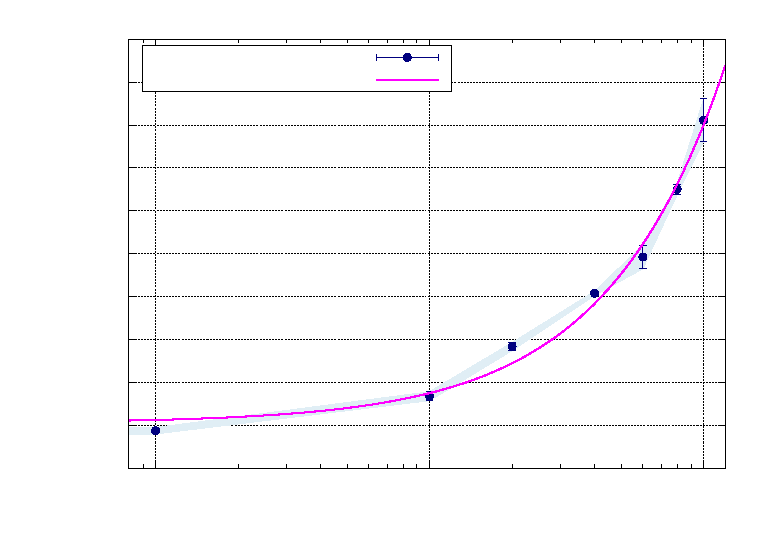
\includegraphics[width={360.00bp},height={252.00bp}]{./1000_e_I_fit}}%
    \gplfronttext
  \end{picture}%
\endgroup
}
        \caption{$e(I)$}
        \label{1000_e_I_fit}
    \end{subfigure}
    \caption{Rhéologies $\mu(I)$, $\Phi(I)$ et $e(I)$ quand $\epsilon_{yy} = 40 \div 60\%$ pour N=1000}
    \label{rheologies_1000}
\end{figure}

\section{Conclusion}\label{discussion}

Les termes dynamiques, sans la partie affine (c'est-à-dire la dérivée de la limite périodique), n'exercent pas d'influence notable sur le frottement au cisaillement dans le VER.
Le comportement de $\mu_{\text{résiduel}}$ obtenu par DEM est cohérent avec les modèles à grande échelle comme attendu.
En revanche, $\mu_{\text{transitoire}}$ est significativement affecté par le nombre de particules.
À notre connaissance, il n'existe pas encore d'étude bibliographique approfondie sur $\mu_{\text{transitoire}}$ ; ce point mérite donc d'être exploré davantage.

\bibliography{bibliographie.bib}

\end{document}